\documentclass[a4paper]{report}
\usepackage[T1]{fontenc}
\usepackage[utf8]{inputenc}
\usepackage[english]{babel}
\usepackage{titlesec}
\usepackage{lipsum}
\usepackage{booktabs}
\usepackage{hyperref}
\usepackage{graphicx}
\usepackage{float}
\usepackage{rotating}
\usepackage[dvipsnames]{xcolor}
\usepackage{enumerate}
\usepackage[shortlabels]{enumitem}
\usepackage{geometry}
\usepackage{pdflscape}
\usepackage{caption}
\usepackage{afterpage}
\graphicspath{{./img/}}

\begin{document}

%%The two following lines remove the line "Chapter n" at the beginning of each chapter, before the title
%\titleformat{\chapter}[display]
%  {\normalfont\bfseries}{}{0pt}{\Large}
\titleformat{\chapter}[hang] 
{\normalfont\huge\bfseries}{\thechapter}{1em}{} 

\title{SafeStreets}
\author{Rosetti Nicola, Sartoni Simone, Torri Vittorio}
\date{date} %%TODO

\begin{titlepage}
\begin{figure}[t]
\centering
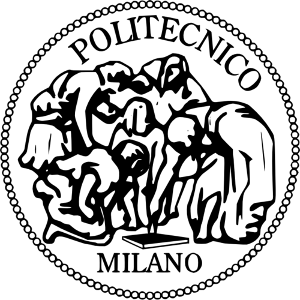
\includegraphics[width=0.3\textwidth]{Logo}
\end{figure}
\begin{center}
    \textsc{ \LARGE{Politecnico di Milano \\}}
	\textsc{ \Large {School of Industrial and Information Engineering\\ }}
	\textnormal{ \Large{Master of Science in Computer Science and Engineering\\}}
	\vspace{3mm}
	\textnormal{ \Large{Software Engineering 2 Mandatory Project\\}}
	\vspace{30mm}
	\fontsize{10mm}{7mm}\selectfont 
    \textup{Safe Streets.}\\
    \textnormal{ \LARGE{Design Document\\}}
\end{center}

\vspace{18mm}

\begin{center}
    \textnormal{\large{\bf Authors:\\}}
	{\large Rosetti Nicola \\ Sartoni Simone \\ Torri Vittorio }
	\fontsize{10mm}{5mm}\selectfont 
\end{center}
\vspace{15mm}

\centering{\large{
Academic Year 2019/2020 \\
\vspace{10mm}
Milano, 09/12/2019 \\
\vspace{2mm}
Version 1.0 
}}

\end{titlepage}

\newgeometry{top=3cm}
\tableofcontents
\listoffigures
\begingroup
\let\clearpage\relax %avoid to put it on a new page
\listoftables
\endgroup
\restoregeometry

\chapter{Introduction}
\section{Purpose}

The purpose of this document is to underline and explain in detail what are the design choices for the deployment of the SafeStreet Application.  The analysis has been made at different levels to underline different views of the same system.
Different levels are identified through the document; here they are just mentioned:
\begin{itemize}
\item the high level architecture;
\item the components that actually builds the system;
\item the deployment view of the system;
\item the messages exchanged among the components and the interfaces they offer;
\item the pattern and technologies exploited for the system;
\item the User Interfaces provided by the system.
\end{itemize}

\section{Scope}
Here the scope of the system is briefly summarized.\\
\textit{SafeStreets} is an application system with the aim to support municipalities in recording parking violations, providing also additional functions for traffic tickets emission, statistics and suggestions.\\
The citizen can use the mobile app to send reports about parking violations, after having been registered, and to consult statistics about violations and accidents.\\
Municipality agents can use the web application to receive the reports by the users, analyze them and possibly emit traffic tickets. They can also consult the previously mentioned statistics.\\
Municipality supervisors can also receive the \textit{suggestions} elaborated by the system to improve the safety on the streets and can also consult reserved statistics, containing personal data about the most egregious offenders.\\
The system is supported by APIs provided by the municipalities and by APIs provided by a map service, as explained in the RASD and in the following sections of this document.
\section{Definitions,Acronyms,Abbreviations}
\begin{itemize}
\item \textit{GPS}: Global Positioning System
\item \textit{HTTPS}: HyperText Transmission Protocol over SSL
\item \textit{API}: Application Programming Interface
\item \textit{MVC}: Model-View-controller pattern
\item \textit{DBMS}: DataBase Management System
\item \textit{DW}: DataWarehouse
\end{itemize}
%\section{Revision History}
\section{Reference Documents}
\begin{itemize}
\item Assignment Document "SafeStreets Mandatory Project Assignment.pdf"
\item RASD Document "RASD1.1.pdf"
\end{itemize}
\section{Document Structure}
The succesive part of th document is divided into 6 chapters:
\begin{itemize}
\item \textit{Chapter 2}: in this chapter all the design choices made during the developmenr of the application presented at different levels of abstraction: from the more general and abstract one concerning tiers and system architecture, to the more technical one, concerning protocols and technologies chosen to deploy the system.
\item \textit{Chapter 3}: in this chapter the user interfaces are presented, using mockups to represent how they should actually be once implemented: different mockups are presented to cover all possible situations worth to be shown.
\item \textit{Chapter 4}: in this chapter the requirements traceability is done. Each requirement described in the RASD is provided by one or more component presented in Chapter 2; in this chapter it's described which components provide what requirements and how this requirement are actually provided.
\item \textit{Chapter 5}: this chapter takes into account how the system is going to be implemented, how the components will be integrated and what strategies of testing is going to be used.
\item \textit{Chapter 6}: this chapter is only meant to show for each component of the group the effort spent, with associated date and hours.
\item \textit{Chapter 7}: in this last chapter are mentioned the references to documents or sites about techologies, pattern and architectures used in this document.

\end{itemize}
\chapter{Architectural Design}
\section{Overview: High­‐level components and their interaction}
The application will be developed using the client-server paradigm on a three-tiered architecture. The three layers of the application (Presentation, Application and Data) are divided into clusters of machines (i.e. tiers) that actually cooperate to provide a specific functionality. In this case we have three tiers  and each tier is responsible for one of the three layers. The client tier is responsible (only) for the \textbf{Presentation} layer; therefore, in this architecture, the thin-client has been adopted considering the fact that the required client-side functionalities are limited. The UIs provided are just meant to show results and to allow clients to choose what they want. In particular there are two types of clients: a \textbf{mobile app} for the citizen which use SafeStreets to report violations and check statistics information and a \textbf{web app} for the police agents and supervisors. \\
The Application tier takes care of the application layer encapsulating all is needed concerning the application logic. It receives the requests from the clients and handles them. It's also responsible for sending asynchronous notifications to the presentation layer when certain conditions are met. It can also filter requests from the clients, deleting invalid ones.\\
The \textbf{Application} tier communicates with the \textbf{Data} tier, responsible for the Data Access layer, that is the layer responsible for accessing the DataBases and performing queries on them.\\
To provide the required functionalities the system exploits also datawarehousing. The DataWarehouse is a component in the Data tier able to deal with historical data and aggregate data taken from the operational databases in a more efficient way than a traditional dbms.
\section{Component view}
In the figure \ref{fig:component-diagram} the \textit{Component Diagram} for the \textit{SafeStreets} system is reported. This is a high level view in which only the main components are immediately shown, while some components will be better detailed afterwards.

\afterpage{
\newgeometry{bottom=2cm}
\begin{landscape}

\begin{figure}[hp]
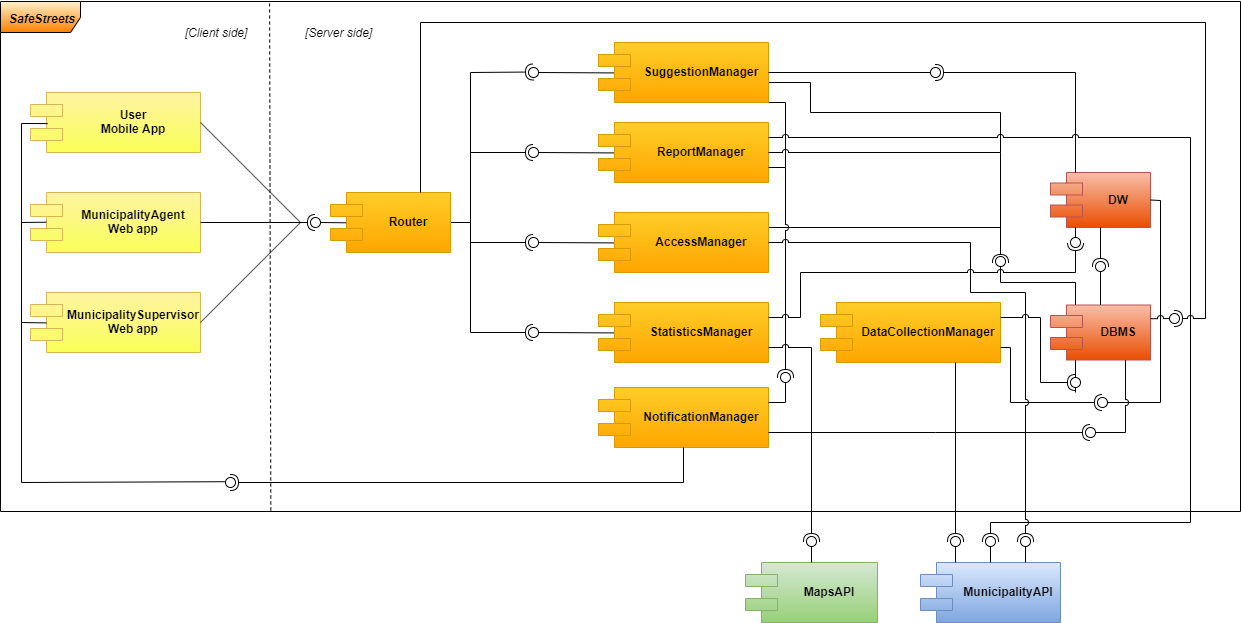
\includegraphics[angle=0, scale=0.55]{Component1}
\caption{UML Component Diagram}
\label{fig:component-diagram}
\end{figure}

\end{landscape}
\restoregeometry
\begin{figure}[hp]
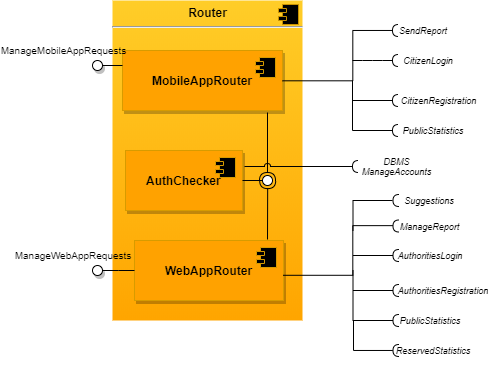
\includegraphics[width=\textwidth]{Router}
\caption{UML Component Diagram for \textit{Router} component}
\label{fig:router-component}
\end{figure}
}
In this diagram when two components can communicate using different interfaces a single interface link is 
reported, for the sake of readability. The various components are now described and detailed:
\begin{itemize}
\item \textbf{Router}: it has the role of dispatching the requests coming from the users applications. Before doing this it has also the important role of verifying the user authentication, checking the token which is sent with all requests performed by an authenticated user. In figure \ref{fig:router-component} a more detailed view is provided, putting in evidence the various interfaces for the mobile and for the web app.

\item \textbf{SuggestionsManager}: this components is the one which elaborates and provides the \textit{Suggestions} for the municipalities. It analyzes the data exploiting the \textit{DataWarehouse} component for the aggregated queries about reports, accidents and tickets and the \textit{DBMS Component} to retrieve non-aggregated information about the streets. It can provide the actual available suggestions for a municipality as an answer to a request coming from the \textit{Router}, but it also notifies the \textit{Municipality Supervisor web app} through the \textit{NotificationManager} component when it discovers a new suggestion (the suggestion discover task is periodically executed, once a month).
\item \textbf{ReportManager}: this component is in charge of all concern the management of the reports sent by the users. It receives them by the mobile application and execute the automatic analysis to identify possible fake reports, it stores them through the \textit{DBMS Component} and it provides the reports to the \textit{Municipality Agents web app}, answering to their requests of confirm/enqueue/discard and allowing them to emit a ticket, exploiting the \textit{Municipality APIs} which provide an interface for this service. Its detailed diagram is shown in figure \ref{fig:reportmgr-component}.

\begin{figure}[htp]
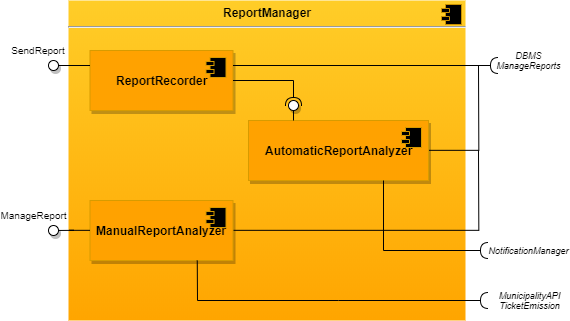
\includegraphics[width=\textwidth]{ReportManager}
\caption{UML Component Diagram for \textit{ReportManager} component}
\label{fig:reportmgr-component}
\end{figure}

\item \textbf{AccessManager}: it manages everything about registration and login of the users. For the citizens registration it calls the municipality service for the verification of identity cards, while for the agents and supervisors registration it calls the municipality service for their identity verification. He stores the accounts data through the \textit{DBMS} component and calls it also to verify the correctness of the login credentials. Once a login has been correctly performed it generates a token, stored in the database and sent back to the user, necessary to perform authenticated requests. This component is detailed in figure \ref{fig:accessmgr-component}.

\begin{figure}[htp]
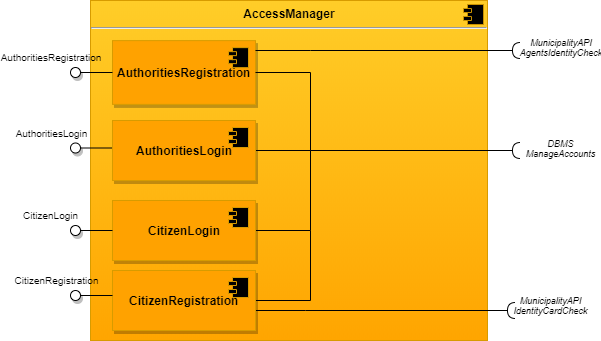
\includegraphics[width=\textwidth]{AccessManager}
\caption{UML Component Diagram for \textit{AccessManager} component}
\label{fig:accessmgr-component}
\end{figure}

\item \textbf{StatisticsManager}: it answers to the statistics requests, both public and reserved, and in doing this it calls the \textit{DataWarehouse} component. It is shown in the diagram in figure \ref{fig:statisticsmgr-component}.

\begin{figure}[htp]
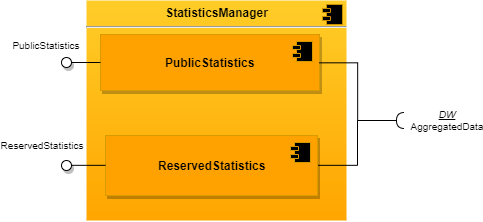
\includegraphics[width=\textwidth]{StatisticsManager}
\caption{UML Component Diagram for \textit{StatisticsManager} component}
\label{fig:statisticsmgr-component}
\end{figure}

\item \textbf{NotificationManager}: this component is the one able to send push notifications to the user clients, both mobile apps and web apps. It is exploited by the \textit{SuggestionManager} and by the \textit{ReportManager}.

\item \textbf{DataCollectionManager}: this component periodically retrieves the data made available by the municipality about accidents, tickets and street characteristics. These latter are stored in the operational database, while the others are retrieved as aggregated data and so are directly stored in the datawarehouse.

\begin{figure}[htp]
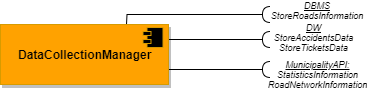
\includegraphics[width=\textwidth]{DataCollectionManager2}
\caption{UML Component Diagram for \textit{DataCollectionManager} component}
\label{fig:datacollectionmgr-component}
\end{figure}

\item \textbf{DBMS}: this component manages the operational database, the main base for the functions of SafeStreets, being in charge of reports, users and streets data.

\item \textbf{DataWarehouse}: this component manages the datawarehouse, the secondary database for the system, used to answer aggregate queries for statistics and suggestions. It is periodically alimented with the dbms data and with the already aggregated data coming from the municipality through the \textit{DataCollectionManager} component.

\item \textbf{MunicipalityAPI}: this is an external component, managed by the municipalities (an instance for each of them which supports the system), whose interface is standardized as described in the \textit{Components Interfaces} section. It is necessary to retrieve the data for building statistics and suggestions, to verify the users identity and to have the possibility of traffic ticket emission through SafeStreets.

\item \textbf{MapsAPI}: this is an external component which is exploited to obtain maps, which will be shown with the associated statistics data.

\item \textbf{UserMobileApp}: this component entirely resides in the \textit{Presentation layer} and it's just an interface to allow the users to use SafeStreets on their mobile devices, sending reports and retrieving statistics information. It performs only minimal controls on the forms before sending them (ex: they are not missing mandatory field) and attaches the user GPS positon.

\item \textbf{AgentWebApp}: this component is the \textit{Presentation layer} of the web app which allows agents to see the reports, analyze them, emit tickets and retrieve users data.

\item \textbf{SupervisorWebApp}: this component is the \textit{Presentation layer} of the web app which allows supervisors to see the reports, possibly analyze them, retrieve all type of statistics and receive the suggestions elaborated by the system. 



\end{itemize}

\section{Deployment view}

So far, only an abstract and general view of the system has been provided. In this section a better detailed view of the system shows how the component previously described are actually deployed in different machines and how each tier is organized.
Here in figures \ref{fig:deployment-diagram} and \ref{fig:architecture-diagram} follow two diagrams: the first one is an UML Deployment Diagram which shows the allocation of the software components in the physical tiers of the system, while the second one is an informal diagram which shows more in detailed the network configuration of the system, with hardware devices such as firewalls and load balancers which are not related to the general architecture but are involved in assuring the proper working of the system. 

\begin{figure}[htp]
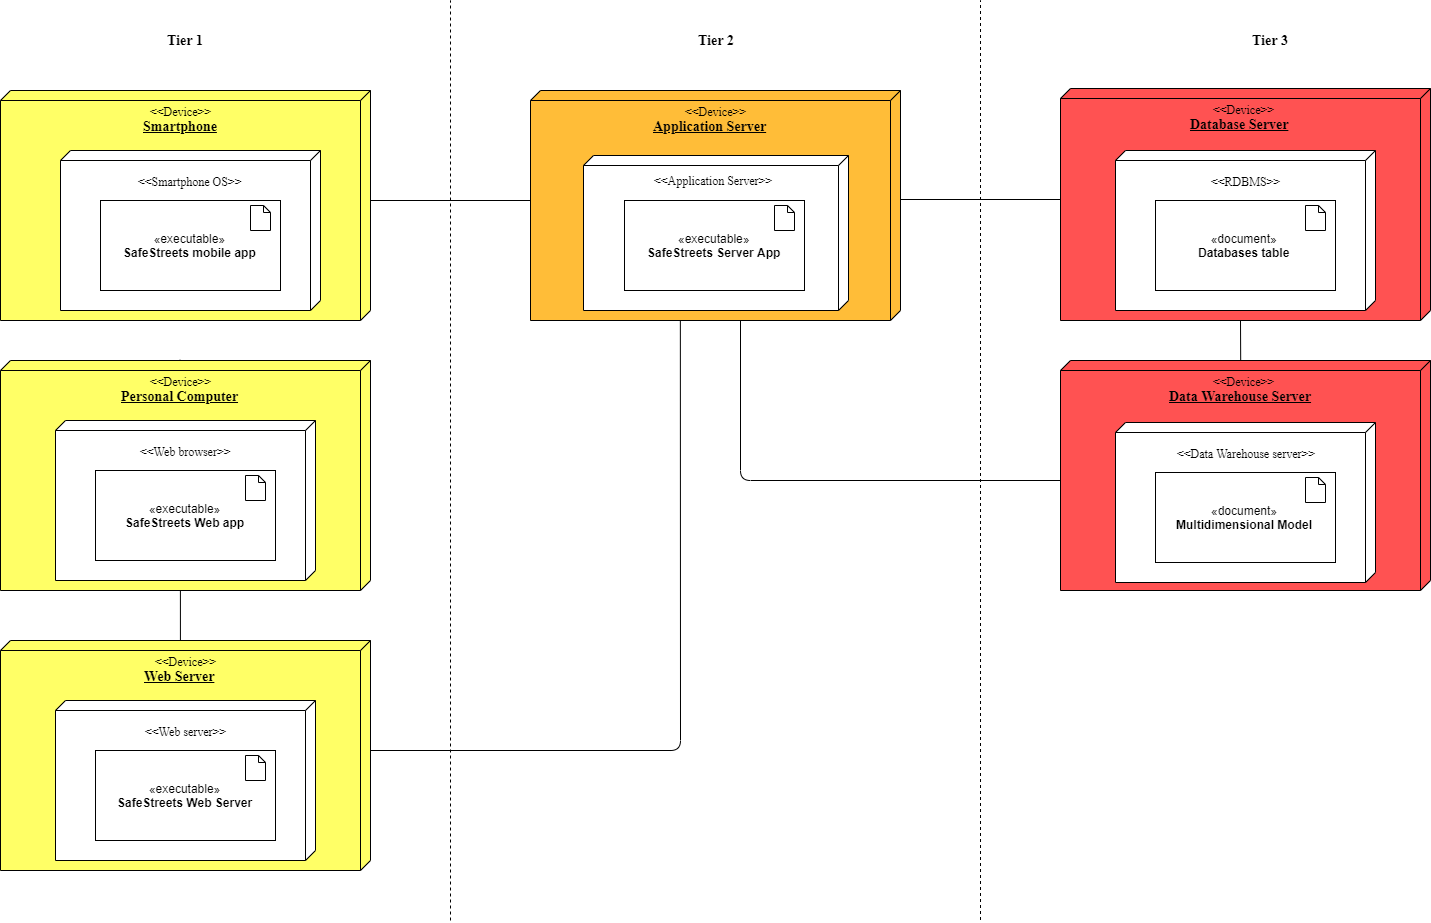
\includegraphics[scale=0.3]{DeploymentDiagram}
\caption{UML Deployment Diagram}
\label{fig:deployment-diagram}
\end{figure}

W.r.t to the component diagram (figure \ref{fig:component-diagram}), the different colors indicate the allocation of components.
For the presentation tier clearly the \textit{smartphones} contain the \textit{UserMobileApp} while the \textit{personal computers} and the \textit{web server} contain the \textit{Municipality Agent WebApp} and the \textit{Municipality Supervisor Web App}.\\
All application logic components (orange in the \textit{Component Diagram}) are deployed on the \textit{Application Server}, while the \textit{DBMS} component is deployed on the \textit{DataBase server} and the \textit{DataWarehouse} component is deployed on the \textit{DataWarehouse server}.

\begin{figure}[htp]
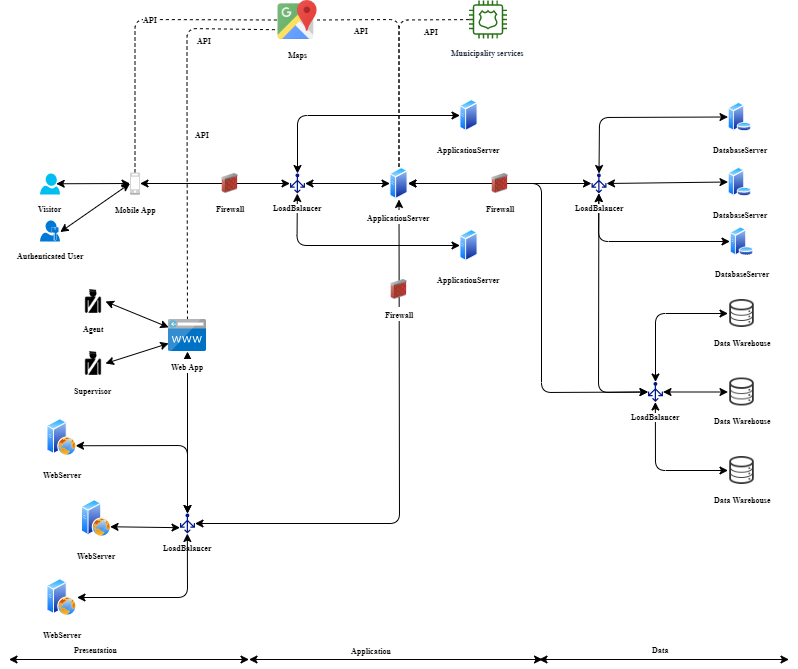
\includegraphics[scale=0.55]{SystemArchitecture}
\caption{Informal architectural view of the system}
\label{fig:architecture-diagram}
\end{figure}
In the \textit{Mobile App} case the client contains all the \textit{presentation layer} while in the \textit{WebApp} case the layer is splitted between the \textit{Web App} and the \textit{WebServer}; the \textit{WebServer} is responsible for contacting the application server and forward the client requests and responses.\\
All the servers are multiplied, cooperating together to improve performance, scalability, fault tolerance and availability. An elastic component (i.e. load balancer) is used to rule the accesses to different applications, dinamically balancing the load among all the Servers. The same is for the data servers.
Each data server is associated with a single replica of the data and exploits the DBMS technology to access the \textit{Database}. The \textit{Database} is fully replicated in different nodes. Techniques and protocols are used to ensure consistency among replicas: they will be full explained in \textit{Other design decisions} section.\\
To ensure and improve security firewalls are installed before and after the application servers to filter accesses from external and unsafe networks. By the creation of a \textit{DMZ} (demilitarized zone) external entities can only have access to the exposed services. They will be properly configurated to allow only legit requests coming from the Application Servers to reach the Data Servers. All the communications will exploit the HTTPS protocol, while unsafe communications will be refused by the firewalls. Security is crucial because the application works mainly with sensible information. 
\section{Runtime view}
In the figures \ref{fig:seq-sendReport}, \ref{fig:seq-userLogin}, \ref{fig:seq-checkReport}, \ref{fig:seq-checkStats}, \ref{fig:seq-register} and \ref{fig:seq-suggestions} some architectural sequence diagrams are provided, showing the interactions among the different components in the execution of various functions of the systems. \\
The \textit{NotificationManager} always requires an interaction with an external server (\textit{Google Firebase Cloud Manager} for Android and Chrome, \textit{Apple Push Notification Service} for iOS), but in the following diagrams it will never be represented, assuming it as internal to the component, for the sake of simplicity and readability. 
\afterpage{
\newgeometry{left=0.5cm, bottom=2cm}
\begin{landscape}
\begin{figure}[hp]
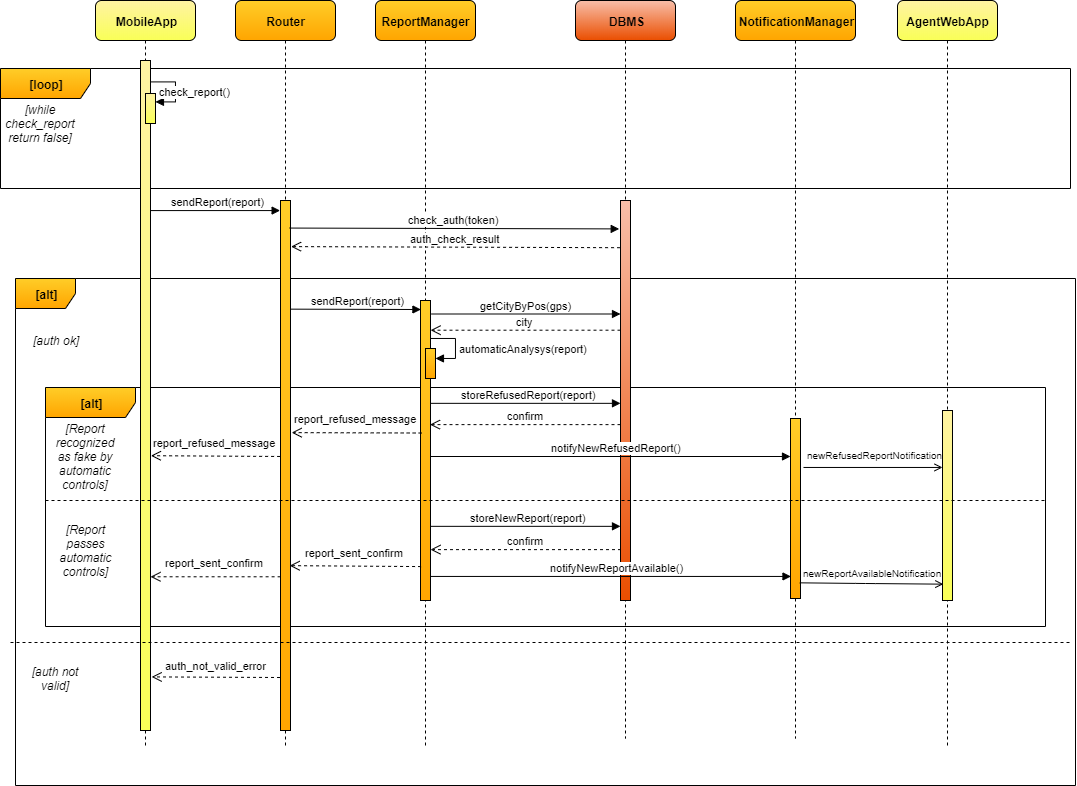
\includegraphics[angle=0, scale=0.70]{ArchSequenceSendReport2}
\caption{UML Architectural Sequence Diagram for \textit{SendReport} use case}
\label{fig:seq-sendReport}
\end{figure}

\end{landscape}
\restoregeometry
}\\\\
In the sequence diagram of figure \ref{fig:seq-sendReport} is shown what messages are actually exchanged among components to process correctly a report send by a User. The User, through the \textit{\textbf{Mobile App}}, fills the report form and sends it to the server for a confirm. The request is handled at first by the \textit{\textbf{Router}} that checks if the User is correctly authorized (i.e. verifies if the corresponding token has the rights needed): if the check is negative, then the request is discarded, otherwise the \textit{\textbf{ReportManager}} calculate the municipality in charge for a specific report comparing the GPS position of the report with the ones associated to municipalities borders in the database. After this, the \textit{\textbf{ReportManager}} checks internally if the pictures in the report have been modified or not. If so, the report is stored as \textit{Refused} and the \textit{\textbf{Notification Manager}} will send a notification about the refused report to the involved \textit{\textbf{MunicipalityAgent Web App}}. If the pictures are not fake then the report is stored as \textit{New report} and the \textit{\textbf{NotificationManager}} will be in charge of notifying the \textit{\textbf{Municipality Web App}} about the new pending report.\\
It has been assumed that the \textit{getCityByPos} request to the \textbf{\textit{DBMS}} returns a city for which the \textit{SafeStreets service} is active. In effect the mobile app should not allow the user to send a report for a city in which the system is not active.
\afterpage{
\begin{landscape}
\begin{figure}[hp]
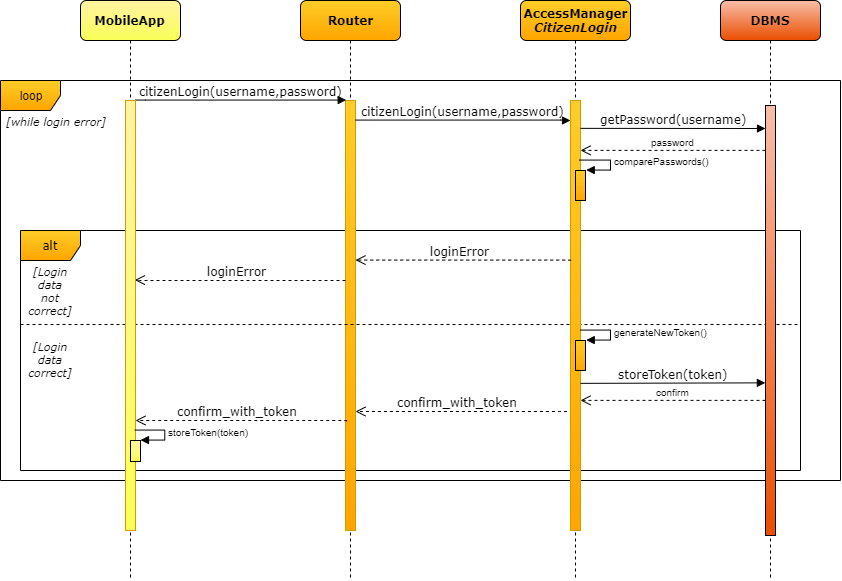
\includegraphics[angle=0, scale=0.70]{ArchSequenceUserLogin}
\caption{UML Architectural Sequence Diagram for \textit{UserLogin} use case}
\label{fig:seq-userLogin}
\end{figure}
\end{landscape}
}\\\\
In the sequence diagram of figure \ref{fig:seq-userLogin} are described the components involved in the user login and their interaction. The User fills the spaces in the \textbf{\textit{Mobile App}} inserting his username and password. The login request is then sent to the \textbf{\textit{Router}} that forwards the message to the \textbf{\textit{AccessManager}}. In particular the subcomponent \textbf{\textit{CitizenLogin}}  handles the login, asking the \textbf{\textit{DB}} the password corresponding to the specified username. After having received the password, it internally checks if  the two passwords (the one coming from the user and the one stored) coincide: if so, the user is successfully logged in and this is notified back to the client, showing him the main page of the App; if not, a notification is sent back to the client, showing him an error message and asking him to insert again username and password. Notice that everytime a new login is performed a new token is generated associated to the specific logged client.
\afterpage{
\newgeometry{left=0.5cm,right=0.5cm,bottom=3cm}
\begin{figure}[hp]
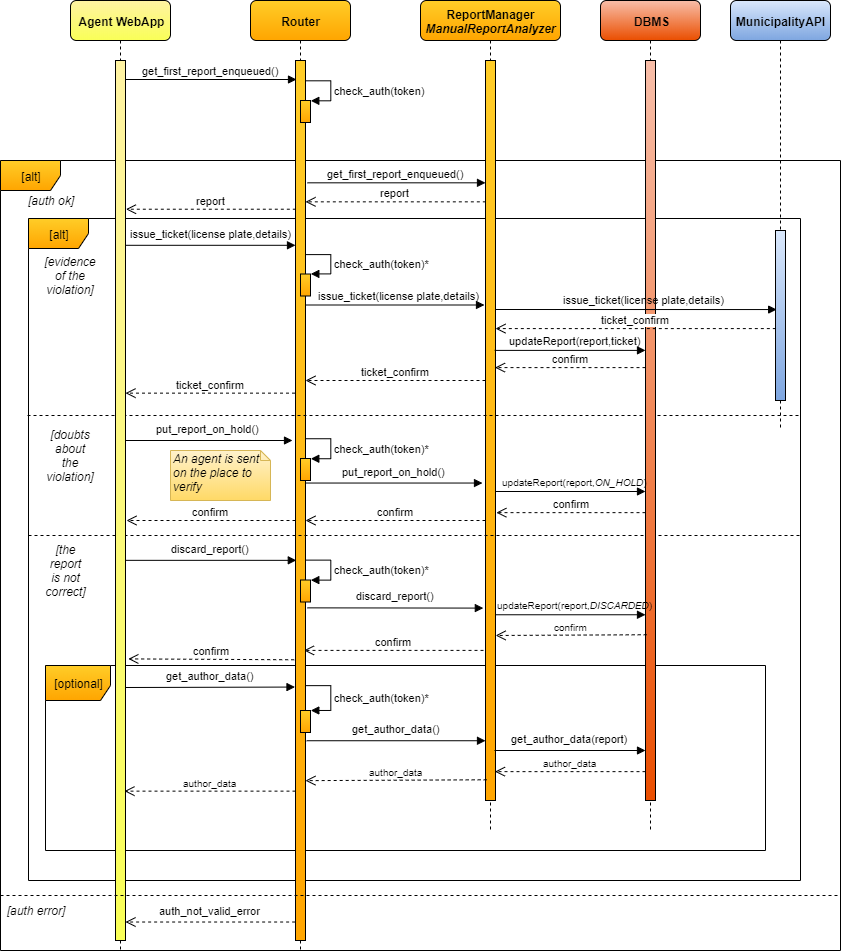
\includegraphics[width=\textwidth]{ArchSequenceAgentCheckReport}
\caption{UML Architectural Sequence Diagram for \textit{AgentCheckReport} use case}
\label{fig:seq-checkReport}
\end{figure}
\restoregeometry
}\\\\
In the sequence diagram of figure \ref{fig:seq-checkReport} is shown the managing of a \textit{Report} by an \textit{Agent}. The request of showing the first report to be analyzed comes from the \textit{\textbf{Agent WebApp}} and is received by the \textit{\textbf{Router}} component, which verifies the authentication and forwards it to the \textit{\textbf{ReportManager}} (in particular the \textit{\textbf{Manual Report Analyzer}} subcomponent). The latter returns the report data to the \textit{\textbf{WebApp}} and then the \textit{Agent} decides what to do. If he wants to issue a ticket the request is sent to the \textit{\textbf{MunicipalityAPI}} and consequently the information is recorded by the \textit{\textbf{DBMS}}.\\
If he decides to put the report on hold, this is simply recorded in the database.
Otherwise if he discards the report this is recorded in the database and he also has the possibility to see the report author's data, always stored in the database.\\
The control for the user authentication is shown for every request, but only the first one presents the \textit{Alternative} choice, for the others, marked with *, it has been assumed a positive answer, for the sake of readability, avoiding to repeat the \textit{Alt} with the error message returned in case of authentication failure. \\
A similar assumption has been made for the municipality answer to the ticket emission request, it has been avoided to report the negative answer, for which the agent would be required to retry the request.
\afterpage{
\begin{landscape}

\begin{figure}[hp]
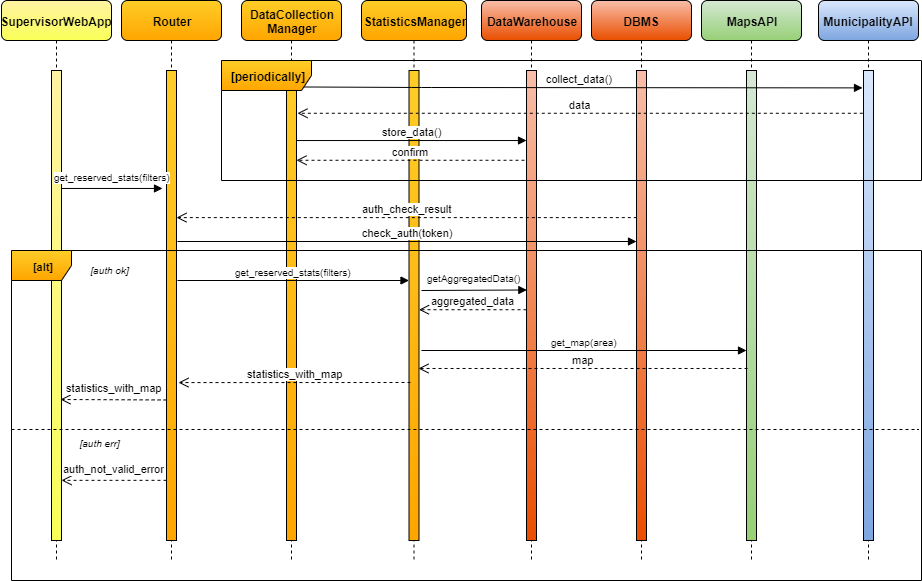
\includegraphics[angle=0, scale=0.70]{ArchSequenceCheckStatistics}
\caption{UML Architectural Sequence Diagram for the \textit{CheckStatistics} use case}
\label{fig:seq-checkStats}
\end{figure}
\end{landscape}
}
\\\\
In the sequence diagram of figure \ref{fig:seq-checkStats} are described the interactions concerning the \textit{Statistics}. Initially is shown how the \textbf{\textit{DataCollectionManager}} component periodically collect data from the \textit{\textbf{MunicipalityAPI}} and stores them. \\
Then is shown the request of \textit{ReservedStatistics} by a \textit{\textbf{Supervisor WebApp}}, with the \textbf{\textit{Router}} which forwards the request to the \textit{\textbf{StatisticsManager}} and this last component that builds the statistics consulting the \textbf{\textit{DataWarehouse}} and the \textit{\textbf{MapsAPI}} to retrieve a map of the interested area.
\afterpage{\newgeometry{left=0.5cm,right=0.5cm,bottom=3cm}
\begin{figure}[hp]
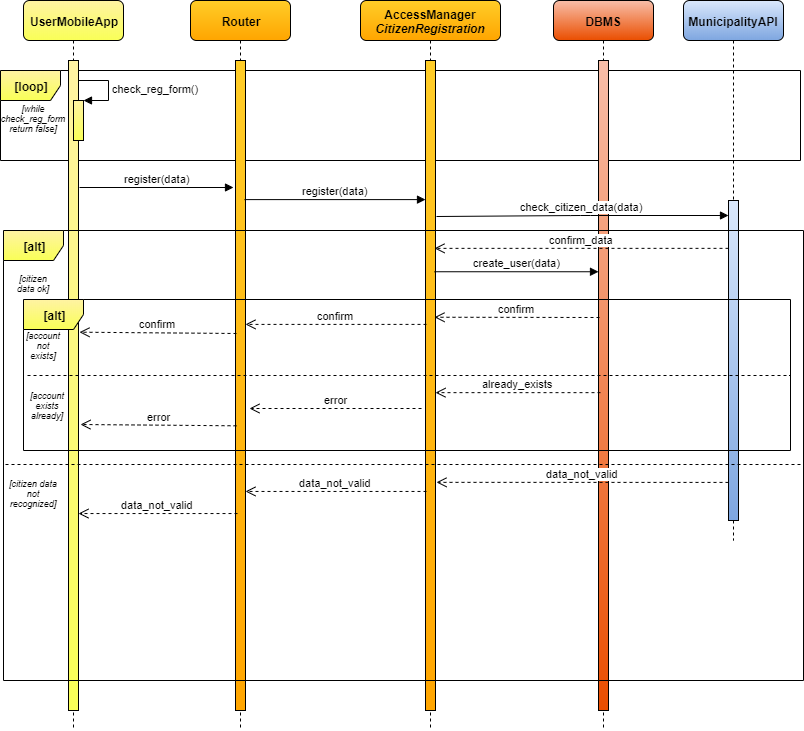
\includegraphics[scale=0.7]{ArchSequenceRegistration}
\caption{UML Architectural Sequence Diagram for \textit{User Registration}}
\label{fig:seq-register}
\end{figure}
\restoregeometry
}\\\\
In the sequence diagram of figure \ref{fig:seq-register} is shown the \textit{Registration} process for a \textit{User}. He compiles the form on the app, which already verifies that all fields have been properly filled, and the app sends the data to the \textbf{\textit{Router}} which forwards the request to the \textbf{\textit{AccessManager}} component (in particular the \textbf{\textit{CitizenRegistration}} subcomponent). This component verifies the correctness of the provided data through the \textbf{\textit{MunicipalityAPI}} and in case of a positive answer store the registration on the \textbf{\textit{Database}}, otherwise it returns an error message.
\afterpage{
\newgeometry{left=1cm,right=1cm, bottom=2cm}
\begin{landscape}
\begin{figure}[hp]
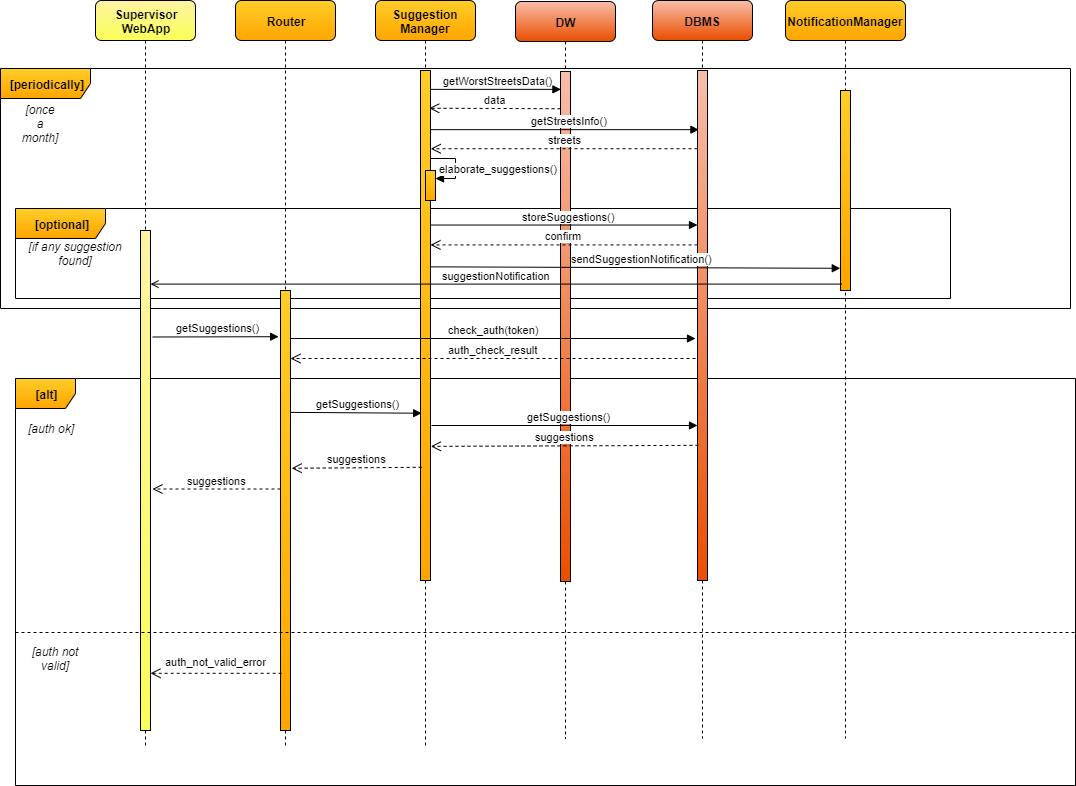
\includegraphics[angle=0, scale=0.65]{ArchSequenceSuggestions}
\caption{UML Architectural Sequence Diagram for the \textit{Suggestions}}
\label{fig:seq-suggestions}
\end{figure}
\end{landscape}
\restoregeometry
}
\\\\
In the sequence diagram of figure \ref{fig:seq-suggestions} are shown the interactions involved by the \textit{Suggestions} function. For first is shown how the \textbf{\textit{SuggestionManager}} periodically retrieve data from the \textbf{\textit{DataWarehouse}} and from the \textbf{\textit{DBMS}} and tries to elaborate new suggestions. If it succeeds in this it stores the new \textit{Suggestion} and sends a notification to the \textbf{\textit{MunicipalitySupervisor WebApps}} through the \textbf{\textit{NotificationManager}}.\\
Then is shown how when a \textit{Supervisor} wants to check the last suggestions, in any moment, he can access them by the corresponding page of his application.


\section{Component interfaces}
\afterpage{
\newgeometry{bottom=2cm}
\begin{landscape}

\begin{figure}[hp]
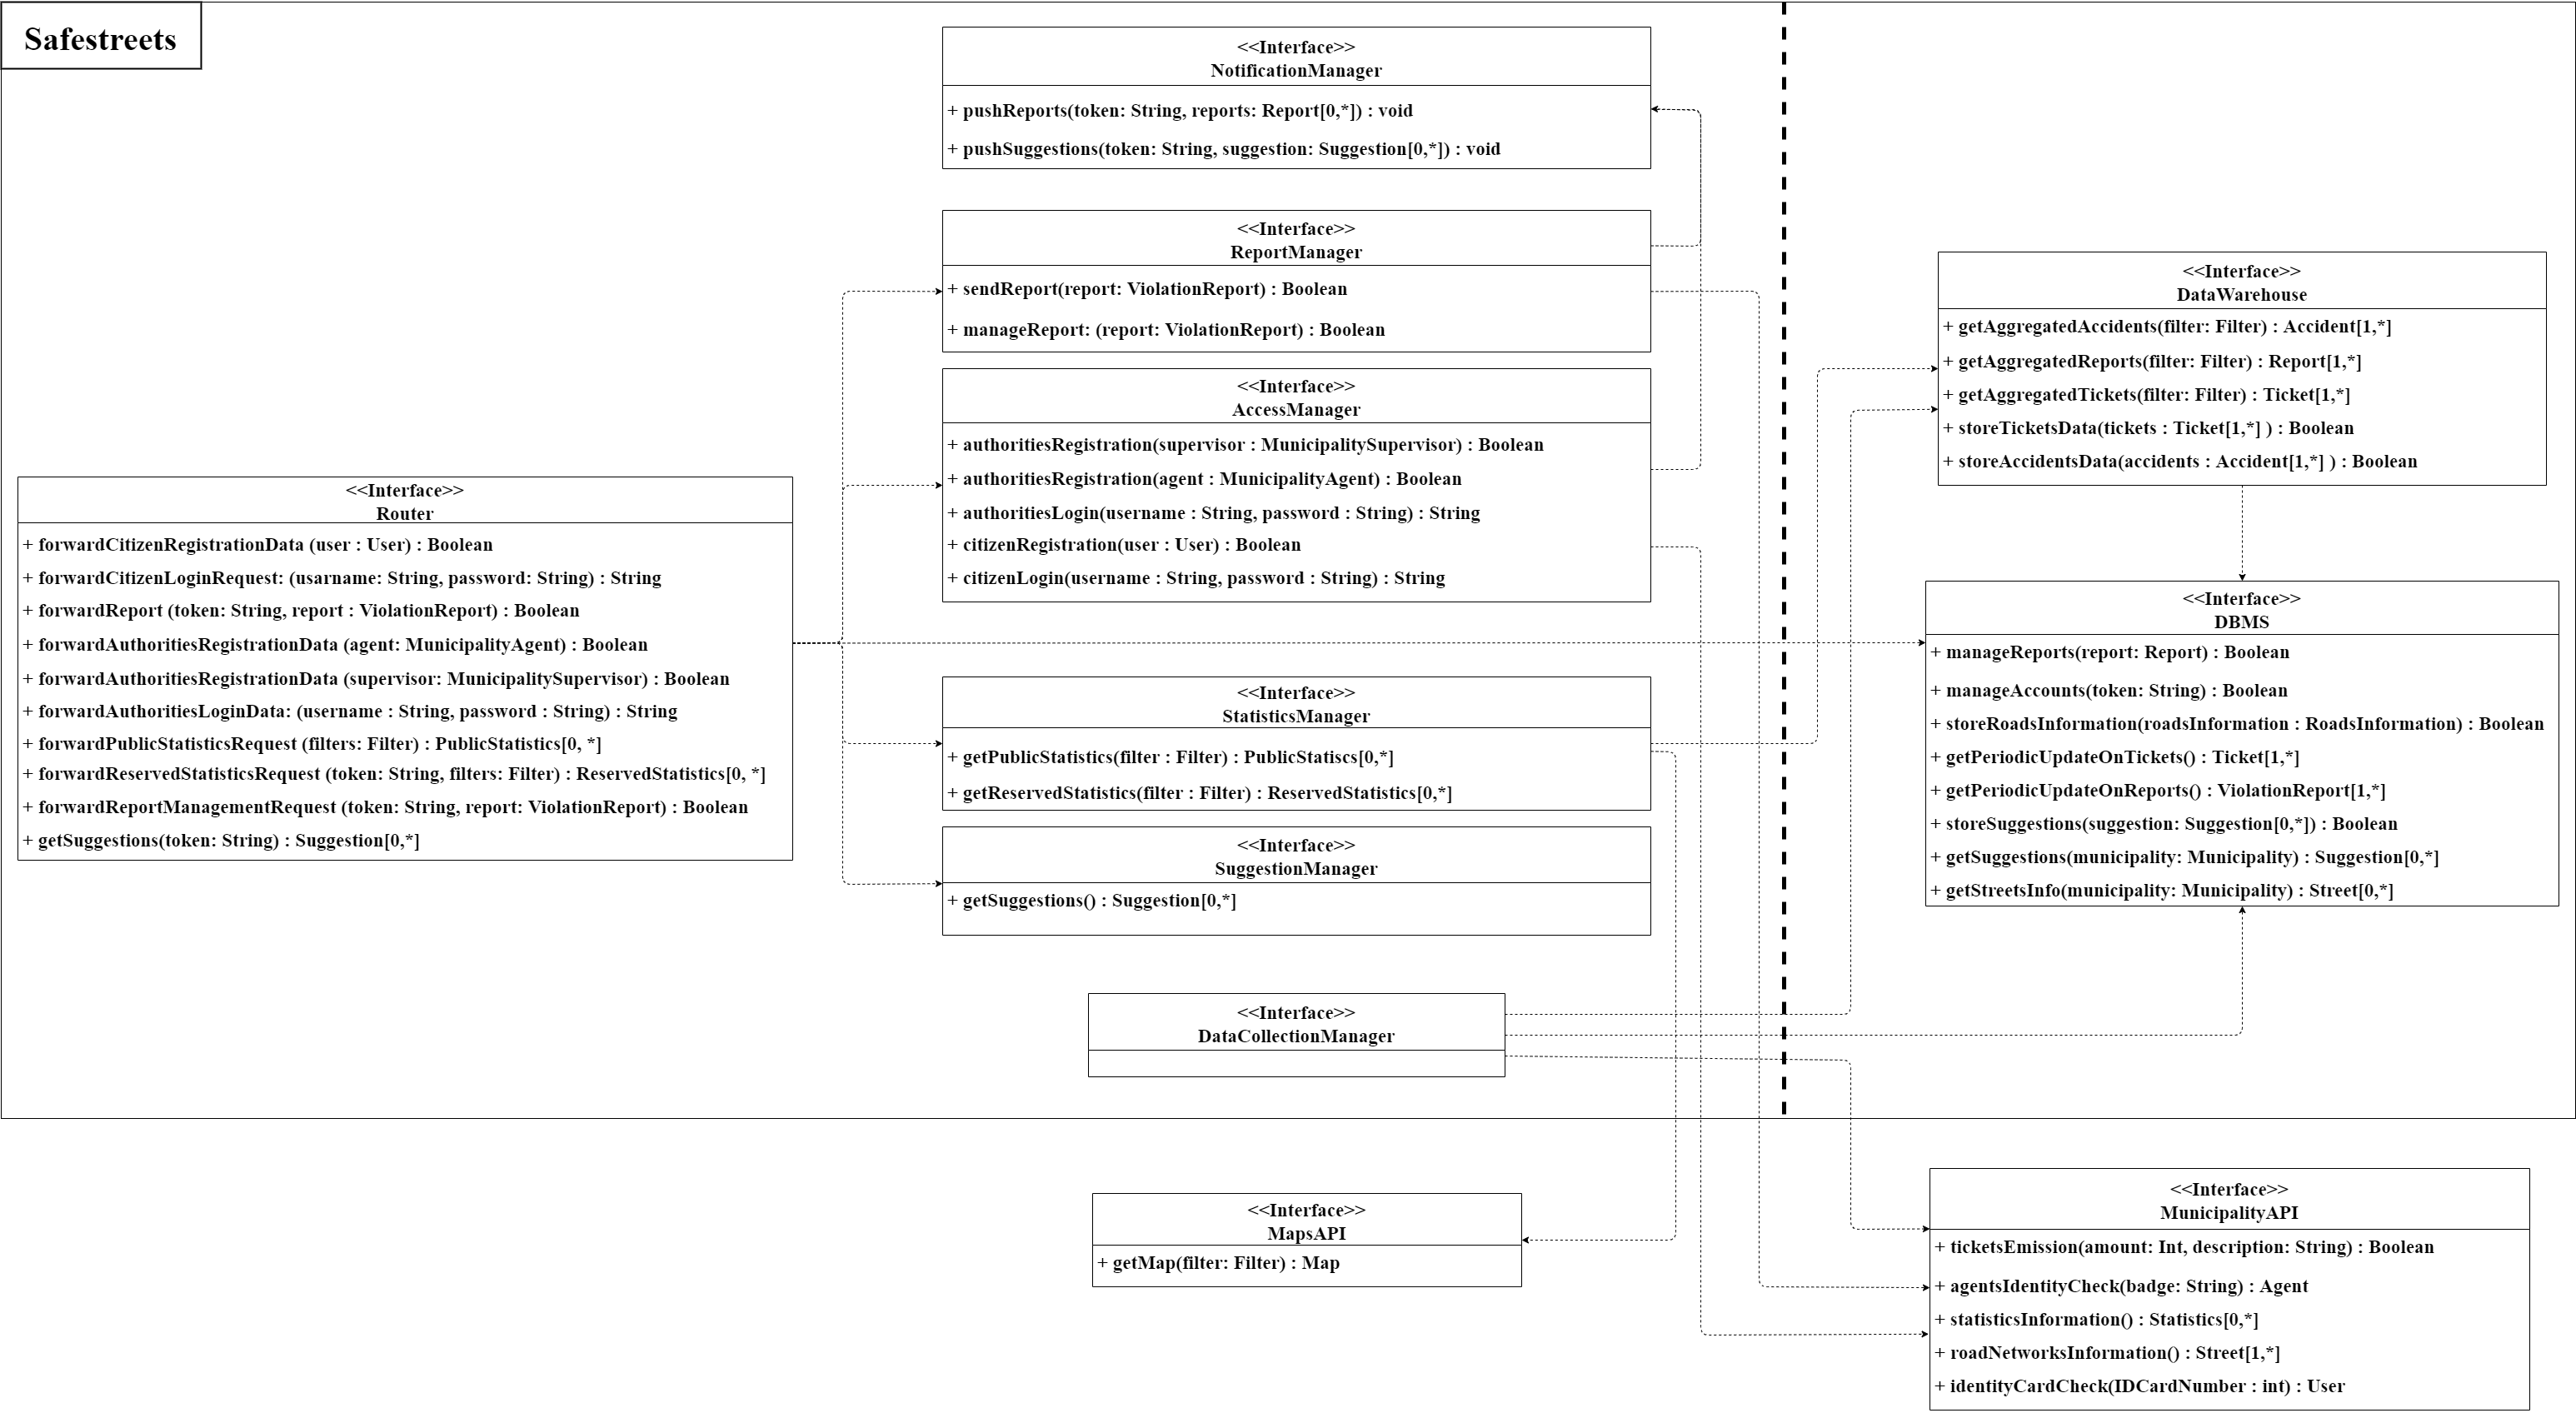
\includegraphics[angle=0, scale=0.25]{Component_Interfaces_Diagram}
\caption{UML Interfaces Diagram}
\label{fig:Interfaces-Diagram}
\end{figure}

\end{landscape}
\restoregeometry
}


In the figure \ref{fig:Interfaces-Diagram} the component interfaces, with reference to what was shown in the Component diagram, are represented. The arrows represent a dependency relation. Each component is described by its invocable methods:
\begin{itemize}
\item Each of invocable methods of the Router are responsable of forwarding a certain request to the associated component; for example ForwardCitizenRegistrationData has one single parameter of User type, which must be forwarded to the AccessManagerComponent, invoking its "citizenRegistration" method.
For all methods which require an authentication the Router checks the authentication of the request with the AuthCheck component, even if its methods are not described in the Diagram because they are internal methods.
\item ReportManager methods can be invoked by the Router when a new Report is sent ("sendReport" method) or an already existing Report must be managed by the responsable agent (ManageReport). In the first case the component will invoke the NotificationManager "pushReports" method, while in the second one it will invoke different MunicipalityAPI methods. In both case it will interact with the DBMS.
\item The methods of the Access Manager are invoked by the Router when it receives a Registration or Login request for a citizen or an Authority. As in the previous component, other methods will be invoked, belonging to the DBMS and the MunicipalityAPI.
\item The methods of the Statistics Manager are invoked by the Router when a request of public or reserverved statistics is asked through the associated method of the Router. The StatisticsManager asks to the Data Warehouse component for tickets, accidents and reports and uses the MapsAPI to provide a map of the interested area.
\item SuggestionManager is only invoked by the Router through its method "getSuggestions", which can return zero, one or more suggestions.
\item NotificationManager provides methods for the AccessManager and the Router and it will invoke the external notification servers methods, not shown here.
\item DataCollectionManager is never invoked by any other component, so its interface does not require any method, infact it is only periodically executed to update data. It obtains data through the MunicipalityAPI with the methods "statisticsInformation" and "roadNetworkInformation" and saves them both in the DataWarehouse, invoking methods "storeTicketsData" and "storeAccidentsData", and in the Database, calling "storeRoadsInformation" method of the DBMS.
\item Data Warehouse provides methods to obtain aggregated data about accidents, reports and tickets, invoked by the StatisticsManager; at the same time data about accidents are updated by the DataCollectionManager and about reports and tickets are updated through two different methods of the DBMS.
\item DBMS provides methods to manage reports and accounts and to store data about roads from the DataCollectionManager. "getPeriodicUpdate" method is invoked by the DataWarehouse to obtain updated data from DBMS.
\item MunicipalityAPI provides methods to emit tickets, to identify both the registrating agent from its badge number and the registrating user from his Identity Card number and to obtain information about statistics and road networks.
\item MapsAPI provides maps according to the filters given as parameter; return value of the API method is "Map" class, which generically denotes the class type for maps and depends on which API has been choosen.
\end{itemize}
In figure \ref{fig:class-diagram} is reported a \textit{Class diagram} which is derived from the class diagram already reported in the RASD with some small modifications. It's still an high level diagram, not necessarily exactly corresponding to the implementation, but it can be a good starting point for the classes to be implemented.
\newgeometry{top=1cm}
\begin{figure}[htp]
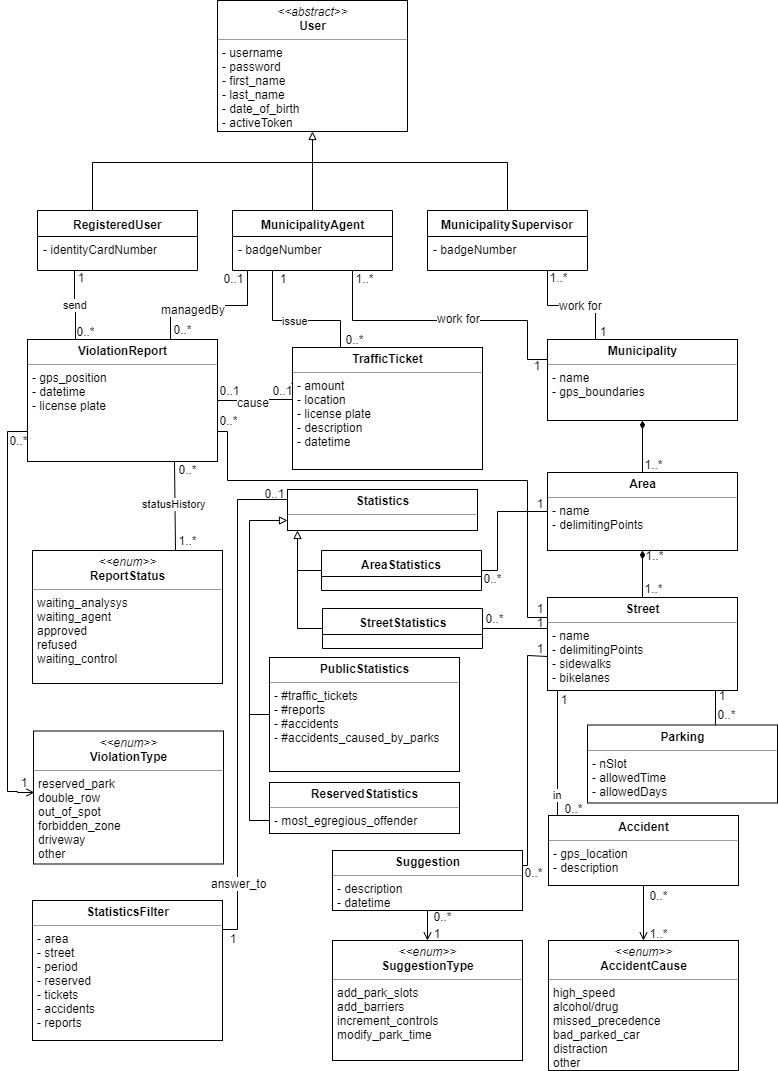
\includegraphics[width=\textwidth]{ClassDiagramDD}
\caption{UML Class Diagram}
\label{fig:class-diagram}
\end{figure}
\restoregeometry
\section{Selected architectural	styles and patterns}
\subsection{Model-View-Controller Pattern}
The (distributed) Model-View-Controller pattern has been exploited to develop the entire application.  This choice has been made to allow fast development, where multiple developers can work together at different levels, and easy debug and update of the application. In section 2.2 the component diagram shows all the high level components that are part of the application. Colors have been used to underline different tiers and so different functionalities: yellow components are View components, orange ones are Controller components and red components are Model Components. For more infos about MVC pattern, see \label{use:MVC-pattern} \hyperref[ref:MVC-pattern]{\textit{[MVC-PATTERN]}}.
\subsection{Facade Pattern}
The facade pattern has been exploited in our application to hide the complexity of the application: only one component can be seen by the client as a "facade", the Router. This component shows an interface that masks all the complexity of the Application and Data Server to the User Interfaces. For more infos about facade pattern, see \hyperref[ref:facade-pattern]{\textit{[FACADE-PATTERN]}} \label{use:facade-pattern}.
\subsection{Publish-Subscribe Pattern}
The publish-subscribe pattern is used for the notification mechanism implemented by the \textit{NotificationManager} component to send notifications to the user applications (both mobile and web) about reports and suggestions. It is based on the functionalities offered by Google and Apple for Android/Chrome and iOS respectively, namely \textit{Google Firebase Cloud Messaging} and \textit{Apple Push Notification Service}. \label{use:pubsub-pattern} See \hyperref[ref:pubsub-pattern]{\textit{[PUBSUB-PATTERN]}} for more information.
\subsection{Thin client}
Our application is based on a three-tier architecture where the client is thin. Thin, in this case, means that client has all (or partial) and only functionalities of the Presentation layer. In particular in this application, client doesn't need to cache anything and doesn't need to know anything about the application logic. No need to store locally statistics, considering that data (and so statistics) can change among two different requests. The client just needs to show the operation that a user can perform and the result of the requests. This is meaningful both for the WebApp and for the Mobile App. 
\subsection{RESTful architecture}
In the system, the REST paradigm has been followed. This choice has been made mainly for the sake of scalability and independent development of different components. This goal has been achieved with uniformity of interfaces , client-server stateless interactions and cacheability of data (meaningful only for Server). For more infos about RESTful architecture, see \hyperref[ref:RESTful-architecture]{\textit{[RESTFUL-ARCHITECTURE]}}. \label{use:RESTful-architecture} \\
\\
Note: here interfaces refers to network interfaces in middleware layer, not to be confused with the component interfaces shown before.
\subsection{Databases}
The operational database of \textit{SafeStreets} is a relational database, considering the structured data it has to manage, regarding users, reports, municipalities. For the statistics and the suggestions elaboration, which require the analysis of a big amount of aggregated historical data, a multidimensional model is used, with a \textit{DataWarehouse}, obtaining its data both from the relational database and directly from the municipality (through the \textit{DataCollectionManager} component). A conceptual description of the databases is present in the \hyperref[sec:db-design]{\textit{Database design}} subsection.
 

\section{Other design decisions}
\subsection{Database design}
\label{sec:db-design}
In figure \ref{fig:er} is shown the \textbf{Entity-Relationship} diagram for the operational database. It is worth to remark that the data coming from the municipality about tickets and accidents are directly stored in the datawarehouse, while here only data about tickets emitted through the SafeStreet system are stored.\\
In figure \ref{fig:dfm} is shown the \textbf{Dimensional Fact Model} for the datawarehouse. The tree facts of interest are Report, Tickets and Accidents. The diagram highlight the dimension of analysis which can be useful for the Statistics and Suggestions functions.
\begin{figure}[htp]
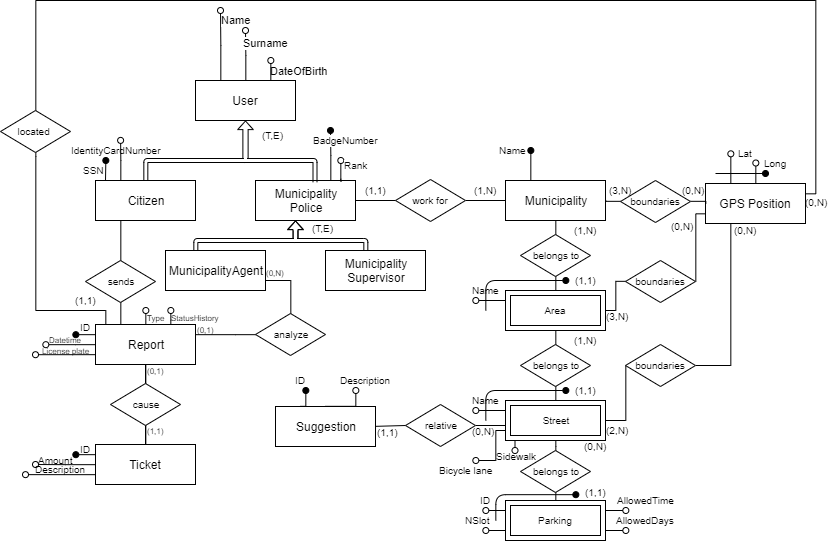
\includegraphics[width=\textwidth]{ER}
\caption{Entity-Relationship diagram for the operational database}
\label{fig:er}
\end{figure}
\begin{figure}[htp]
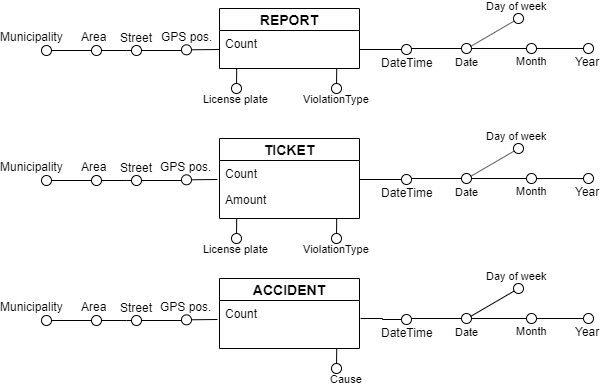
\includegraphics[width=\textwidth]{DFM}
\caption{Dimensional Fact Model diagram for the data warehouse}
\label{fig:dfm}
\end{figure}

\subsection{Consistency and update strategies among replicas}
In this application,  we need a client-centric consistency among replicas because end users (and therefore application servers that act as clients towards the DataServers) don't always connect to the same DataServer, due to the presence of the load balancer. Every DataServer can respond to a request to read or write data so we use an active replication protocol. In particular we exploit leaderless replication in which the decision on the value to read and the write to perform is decided by all the replicas or at least a quorum of them. The type of chosen consistency model  is the "read your writes": the effect of a write operation by a process on a data item x will always be seen by a successive read operation on x by the same process. 
Concerning the update propagation we opted for propagating a notification of the operation, assuming that there will be more writes than reads.  The propagation strategy chosen is the Gossiping strategy: when a replica is updated then it just propagates that update to all the nodes that it knows; if a replica receives an update that it has already received then the probability of propagating that information is decreased on that replica. 

\chapter{User interface design}
In this chapter are presented again mockups shown in the RASD with a few additions (figure from \ref{fig:initial-page} to \ref{fig:mock-webregister} ).\\
\afterpage{
\begin{figure}
\begin{minipage}{.45\textwidth}
\centering
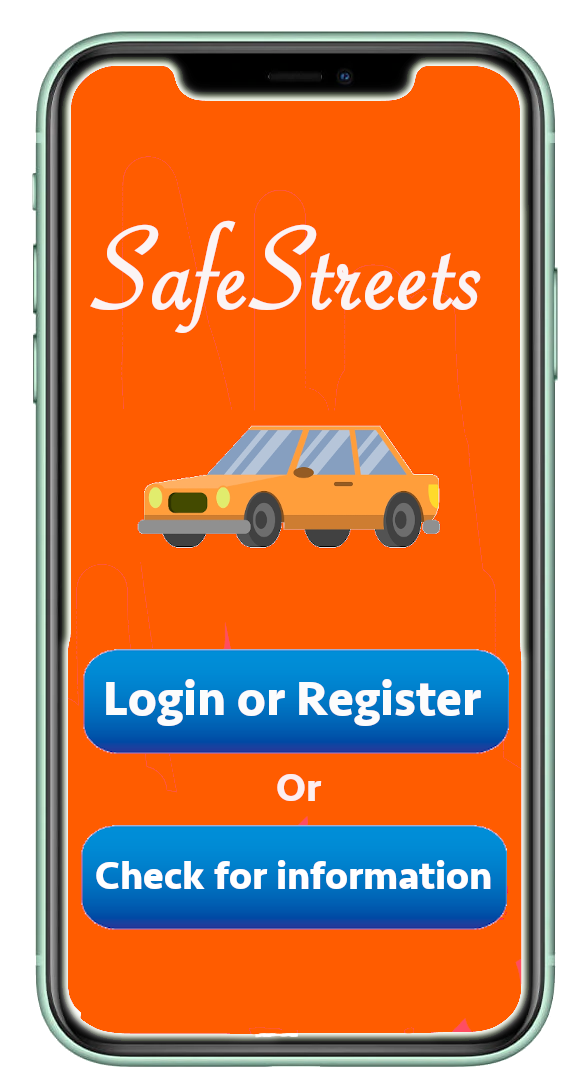
\includegraphics[width=.7\linewidth]{../RASD/img/mockups/phoneschermatainiziale.png}
\caption[Mobile App mockup for initial page]{Mobile App mockup for the starting page after having opened the app for a User}
\label{fig:initial-page}
\end{minipage}\hfill
\begin{minipage}{.45\textwidth}
\centering
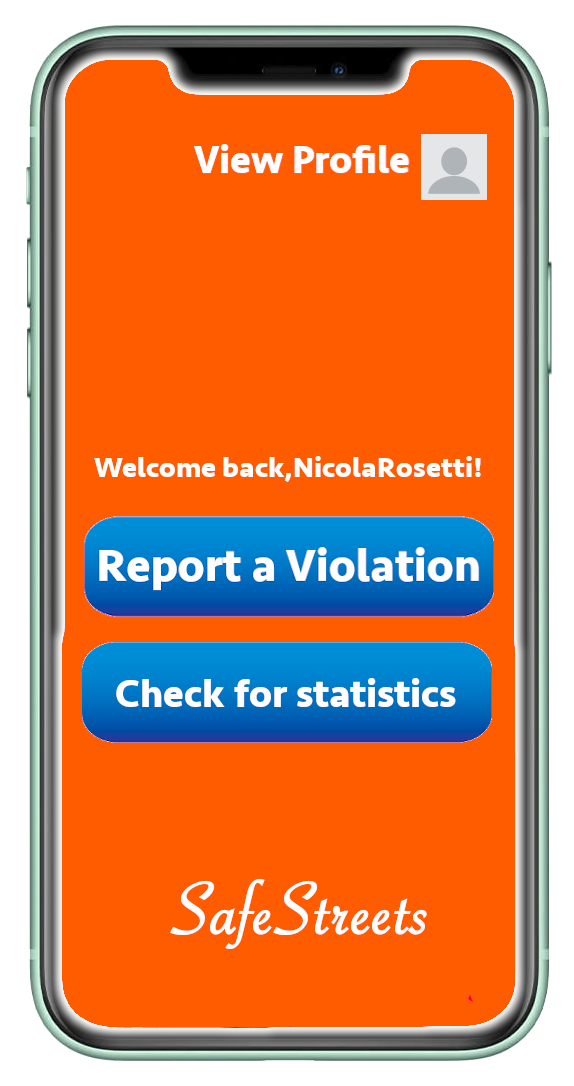
\includegraphics[width=.7\linewidth]{../RASD/img/mockups/Schermata_principale.png}
\caption[Mobile App mockup for main page]{Mobile App mockup for the main page of the application after a User has logged in }
\label{fig:main-screen}
\end{minipage}\hfill
\end{figure}
\begin{figure}
\begin{minipage}{.45\textwidth}
\centering
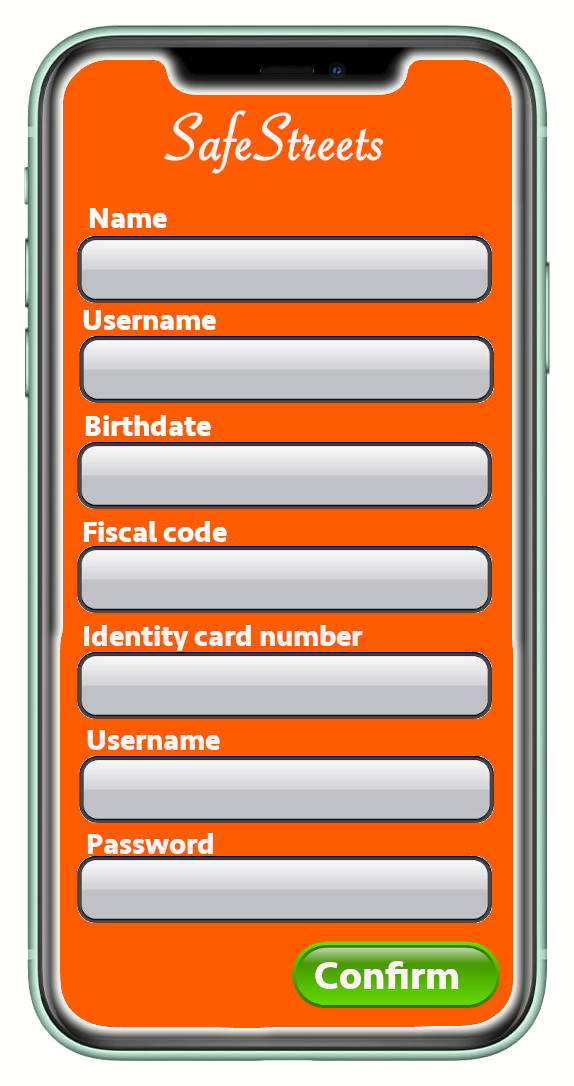
\includegraphics[width=.7\linewidth]{../RASD/img/mockups/Register.png}
\caption[Mobile App mockup for the registration]{Mobile App mockup for a User when he wants to register}
\label{fig:register-page}
\end{minipage}\hfill
\begin{minipage}{.45\textwidth}
\centering
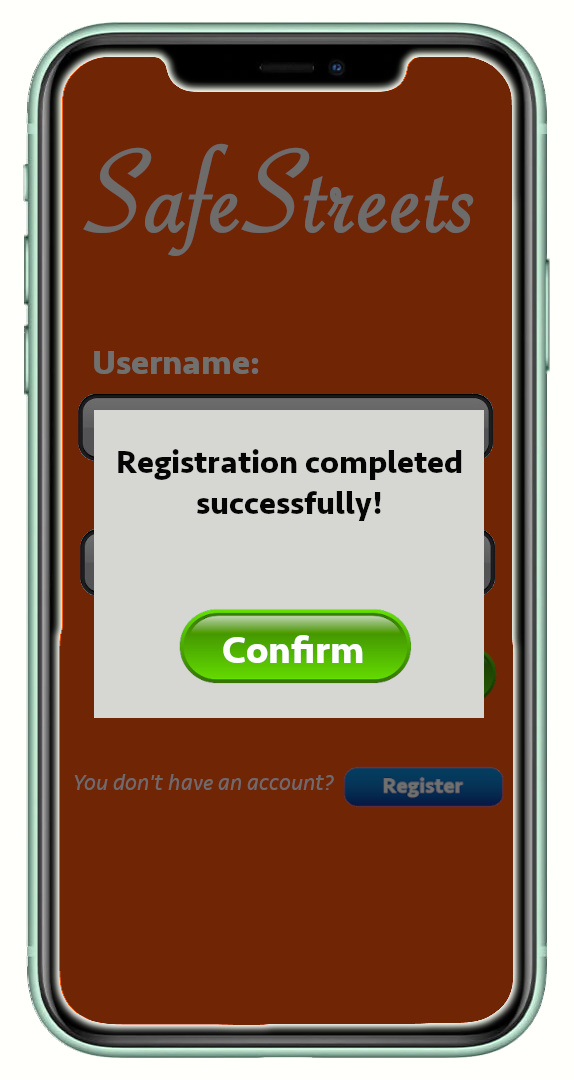
\includegraphics[width=.7\linewidth]{mockups/RegistrationConfirm.png}
\caption[Mobile App mockup for the registration confirm]{Mobile App mockup for the registration confirm popup}
\label{fig:register-confirm}
\end{minipage}\hfill
\end{figure}
\begin{figure}
\begin{minipage}{.45\textwidth}
\centering
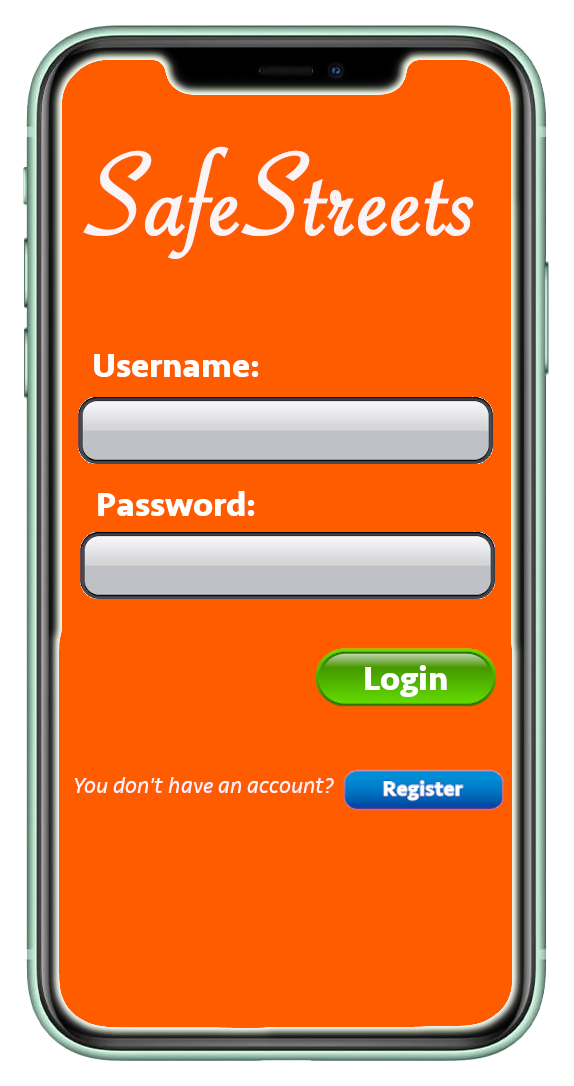
\includegraphics[width=.7\linewidth]{../RASD/img/mockups/loginscreen.png}
\caption[Mobile App mockup for the login screen]{Mobile App mockup interface for the login of a registered User}
\label{fig:login-page}
\end{minipage}\hfill
\begin{minipage}{.45\textwidth}
\centering
\includegraphics[width=.7\linewidth]{../RASD/img/mockups/Report.png}
\caption[Mobile App mockup for the report page]{Mobile App interface mockup for the reporting of a violation for registered Users}
\label{fig:report-page}
\end{minipage}\hfill
\end{figure}
\begin{figure}
\centering
\includegraphics[width=.32\textwidth]{../RASD/img/mockups/Checkstatistics.png}
\caption[Mobile App mockup for statistics]{Mobile App interface mockup for the statistics for Users}
\label{fig:check-statistics}
\end{figure}
\begin{figure}[htp]
\centering
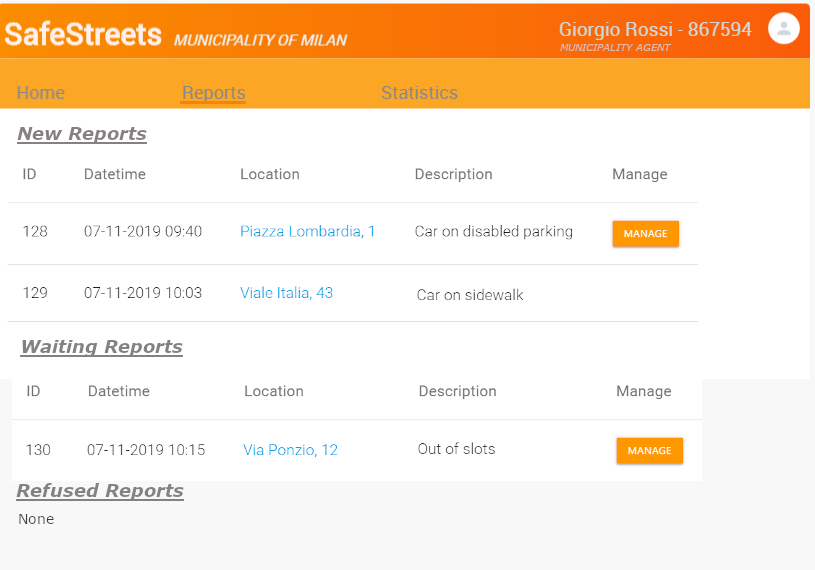
\includegraphics[width= \textwidth]{../RASD/img/mockups/homeReport.png}
\caption[Web mockup for reports page]{Web interface mockup for the report list for a logged Municipality Agent }
\label{fig:mock-webreports}
\end{figure}
\begin{figure}[htp]
\centering
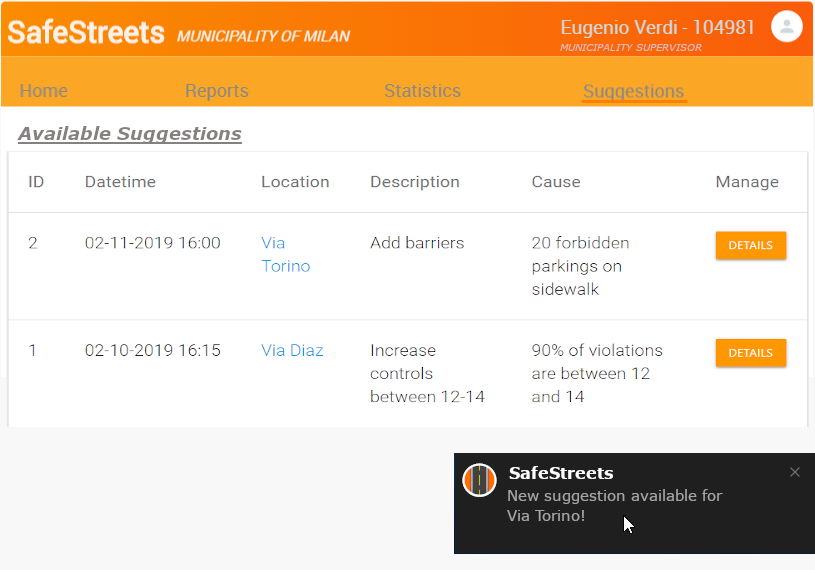
\includegraphics[width= \textwidth]{../RASD/img/mockups/homeSuggestions.png}
\caption[Web mockup for suggestions page]{Web interface mockup for the suggestions list for a logged Municipality Supervisor}
\label{fig:mock-suggestions}
\end{figure}
\begin{figure}[htp]
\centering
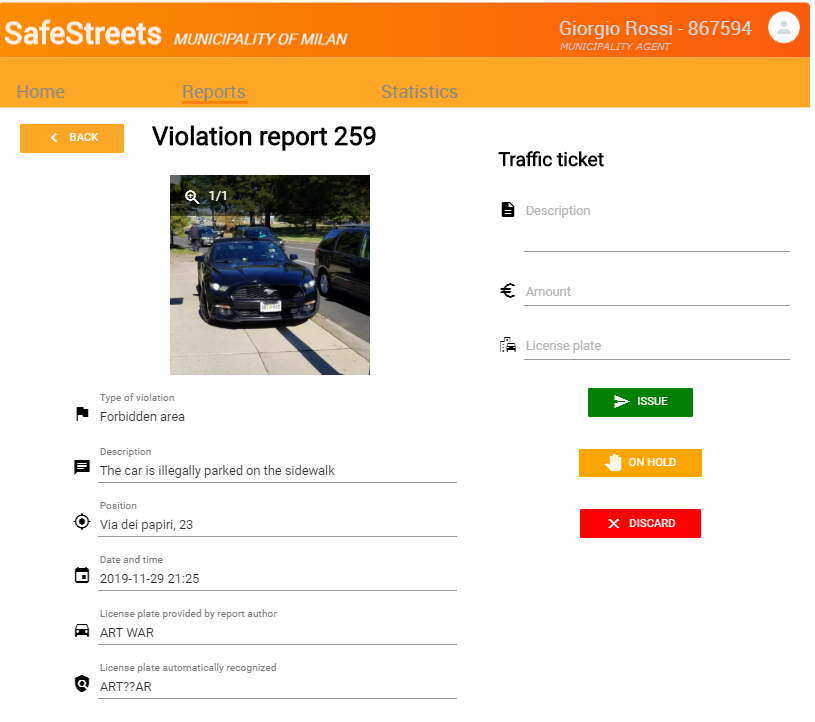
\includegraphics[width= \textwidth]{mockups/reportAnalysis.png}
\caption[Web mockup for the report analysis page]{Web interface mockup for the report analysis page used by Municipality Agents}
\label{fig:mock-reportanalysis}
\end{figure}
\begin{figure}[htp]
\centering
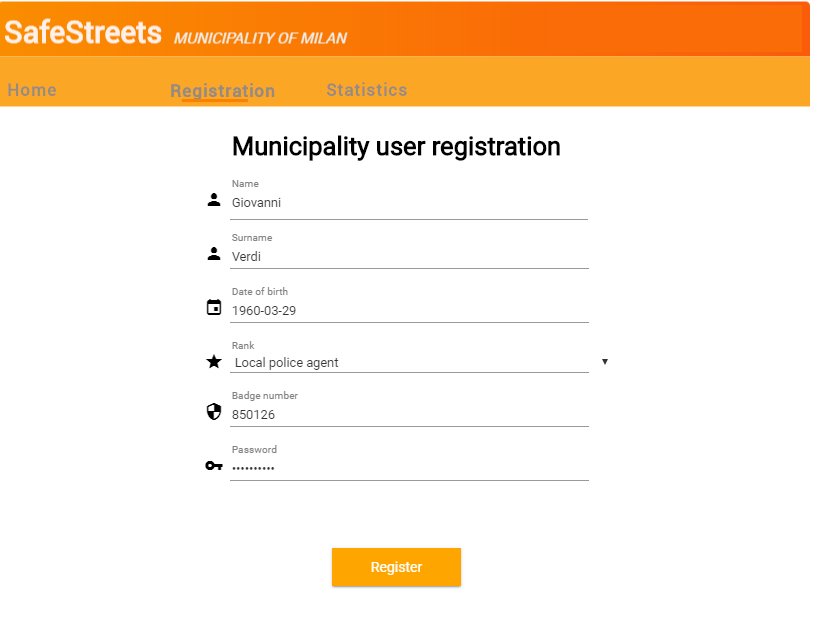
\includegraphics[width= \textwidth]{mockups/municipalityRegistrationMockup.png}
\caption[Web mockup for registration page]{Web interface mockup for the registration page for a municipality user}
\label{fig:mock-webregister}
\end{figure}
}
In the figures \ref{fig:MobileApp-activity}, \ref{fig:SupWebApp-activity} and \ref{fig:AgentWebApp-activity} are shown activity diagrams that describe how a user (citizen, agent or supervisor) can navigate in the UIs offered by the application. The choice of activity diagrams has been made following the suggestions of the paper \label{use:UML-Activity} \hyperref[ref:UML-Activity]{\textit{[UML-ACTIVITY]}}.Notice that  Users and Municipality Agents/Supervisors can quit the application from any state to reach the end state of the diagrams. No end state is represented and so are all the arrows that lead to them; this has been done for the sake of readability of the diagrams.
\afterpage{
\newgeometry{bottom=4cm}
\begin{landscape}
\begin{figure}[hp]
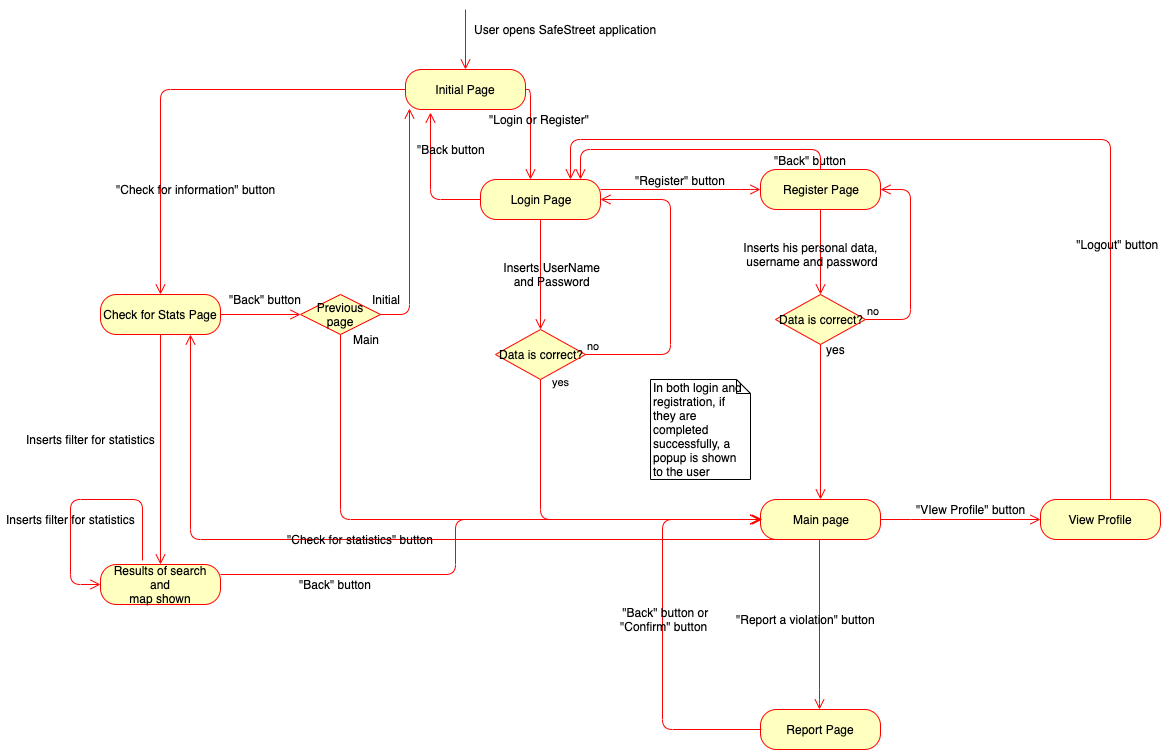
\includegraphics[angle=0, scale=0.50]{Activity_diagram_UI}
\caption{UML Activity Diagram for the User Mobile App navigation}
\label{fig:MobileApp-activity}
\end{figure}
\end{landscape}
\begin{landscape}
\begin{figure}[hp]
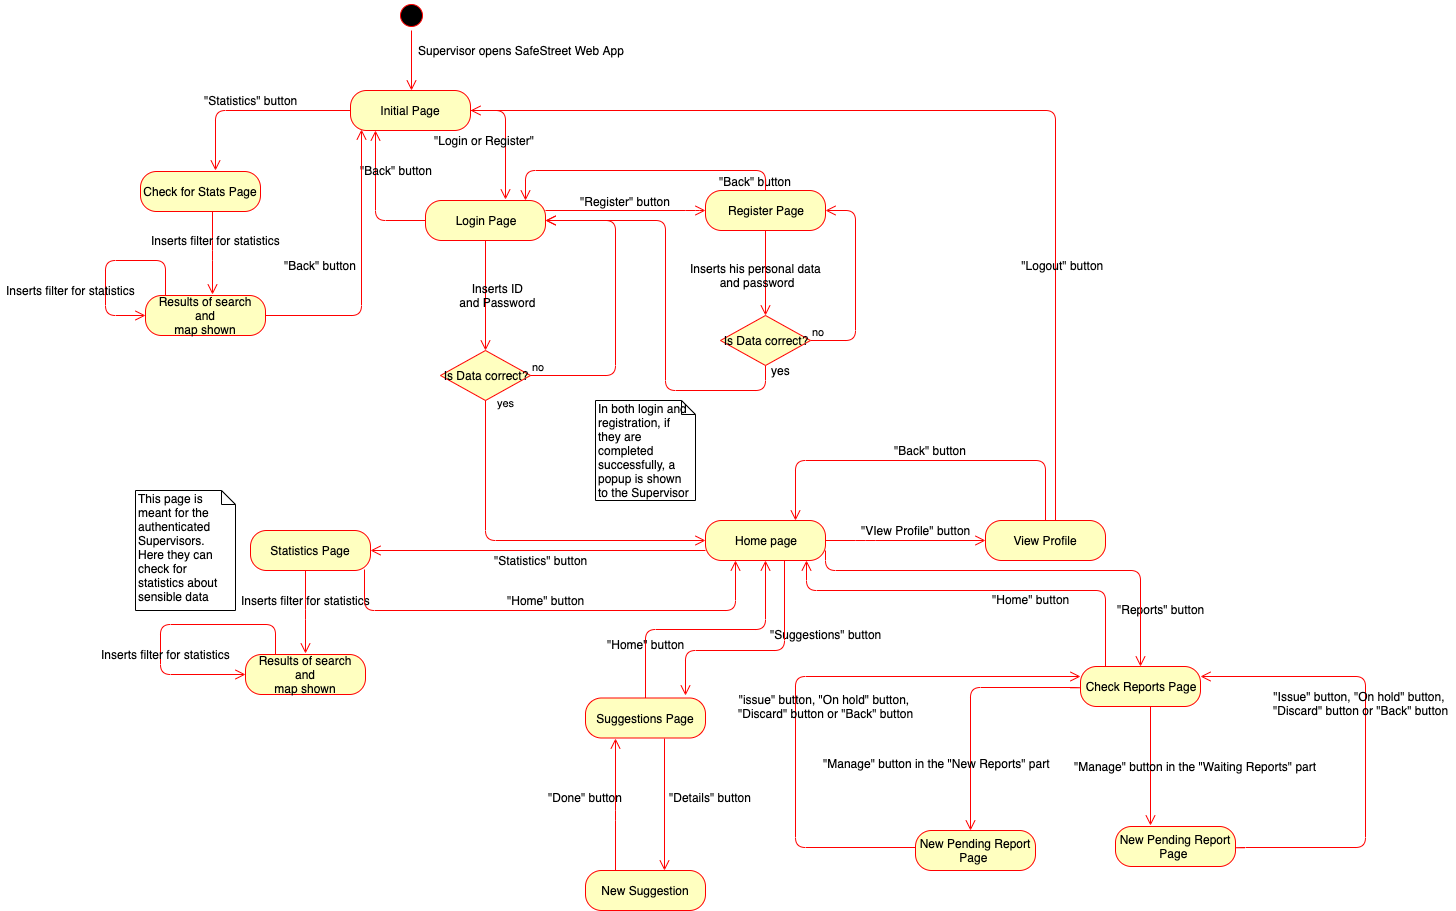
\includegraphics[angle=0, scale=0.50]{Activity_diagram_Supervisor_WebApp}
\caption{UML Activity Diagram for the MunicpalitySupervisor Web App navigation}
\label{fig:SupWebApp-activity}
\end{figure}
\begin{figure}[hp]
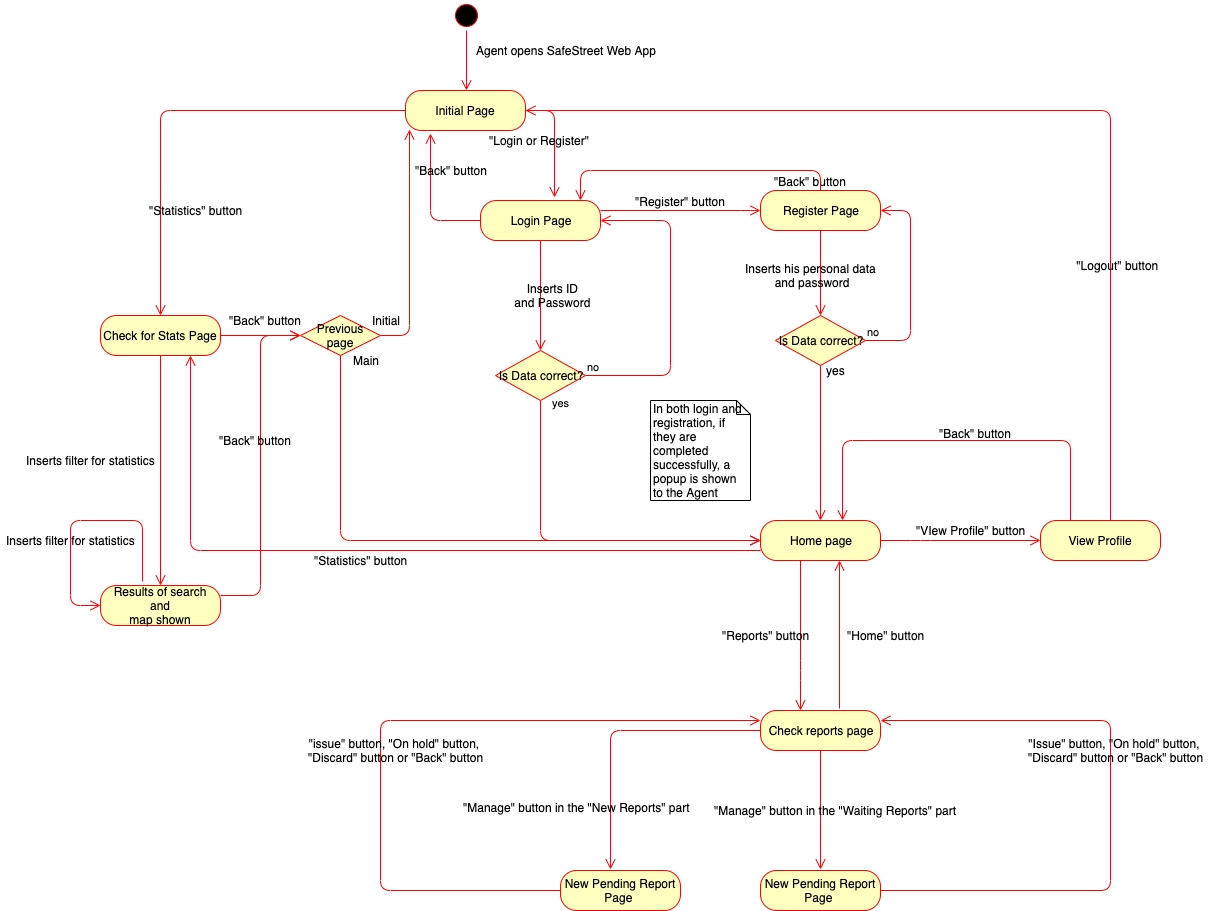
\includegraphics[angle=0, scale=0.50]{Activity_diagram_WebApp}
\caption{UML Activity Diagram for the MunicipalityAgent Web App navigation}
\label{fig:AgentWebApp-activity}
\end{figure}
\end{landscape}
}

\chapter{Requirements Traceability}

In this section is shown how the requirements are actually ensured and which components actually ensure them. It's worth to notice that for the sake of simplicity the Router has been ignored but it's always involved when dealing with a request coming from one of the clients.
Table \ref{tab:req-trace} has been added to highlight for each component what requirements it ensures.
\begin{table}[H]  
  \centering
  \begin{tabular}{|c|c|}
    \cline{1-2}
   	\rule{0pt}{10pt} 
   	\begin{large}
    \textbf{Component} 
    \end{large}&\begin{large}
    \textbf{Requirements} 
    \end{large}\\  \hline
    User Mobile App &  R1,R3, R4, R5, R6, R7, R8, R9, R10, R28, R29, R30, R33, R34,R35\\ \hline
    MunicipalityAgent Web App & R19,R20,R21,R22,R23, R24, R26,R28,R29,R30,R33,R34,R35 \\ \hline
    MunicipalitySupervisor Web App & R28,R29,R30,R34,R35,R36,R37,R38, R40 \\ \hline
    AccessManager & R1, R2, R3, R25, R26, R39, R40 \\ \hline
    ReportManager & R11, R12, R13, R14, R15, R16, R17,R18\\ \hline
    SuggestionManager & R42 \\ \hline
    StatisticsManager & R30, R36 \\ \hline
    NotificationManager & R18, R43 \\ \hline
    DataCollectionManager & R31,R41 \\ \hline
    DataWarehouse & R27, R30, R31, R32, R36, R41, R42, R43 \\ \hline
    
  \end{tabular}
  \caption{Table for mapping requirements to components} \label{tab:req-trace}
\end{table}
In the following lines is explained how the requirements are provided by the components:
\begin{enumerate}[start=1,label={[R\arabic*]}]
\item \label{[R1]} The system must allow people to register to it providing personal data (name, surname, birthdate, identity card number, fiscal code) and selecting a username and a password: this requirement is provided by the \textit{AccessManager} and the \textit{User Mobile App} components. The \textit{User Mobile App} allows the user to fill blank spaces with username and password and the \textit{AccessManager} handles requests of registration from the client.
\item \label{[R2]} The system must verify the correctness of the provided personal data of a registered user checking them from the identity card number, blocking the registration if they are not correct: the \textit{AccessManager} checks the received data from the Client calling the \textit{municipality API services} that actually possesses sensible data of the users. 
\item  \label{[R3]}The system must allow registered users to login through their username and password, if they provide them correctly: this requirement is provided by the \textit{AccessManager} and the \textit{User Mobile App}. The \textit{User Mobile app} allows registered users to insert username and password while the \textit{AccessManager} handles the requests of login from the user and blocks them  if, checking from the DataBase, the inserted data is not correct. 
\item \label{[R4]} The system must allow the logged user to fill a report violation form: this requirement is fulfilled by the \textit{User Mobile App} component that allows the logged user to choose the "Report a violation" feature.
\item  \label{[R5]}The system must let the user select the type of violation detected: the requirement is fulfilled by the \textit{User Mobile App} component, showing an empty space to fill with the type of violation detected in the "Report a violation" process.
\item  \label{[R6]} The system must allow the user to insert the license plate in a violation report:  the requirement is fulfilled by the \textit{User Mobile App} component, showing an empty space to fill with the license plate of the car that committed the violation in the "Report a violation" process.
\item  \label{[R7]}While reporting the violation, the system must allow users to take one or more pictures of the potential violation: the requirement is fulfilled by the \textit{User Mobile App} component, allowing user to click on the "Take a picture" button.
\item \label{[R8]}The system must not allow users to choose pictures not taken in the moment of the report: this requirement is guaranteed by the \textit{User Mobile App} by not allowing client to just pick some random picture from his local storage.
\item \label{[R9]}The system must collect the current position of the user, using GPS: the \textit{User Mobile App} component ensures this requirement by taking the current position of the User using GPS location.
\item \label{[R10]}The system must allow user to confirm or delete the current report: the \textit{User Mobile App} component ensures this requirement by either sending the report for a check through the "confirm" button or deleting the current report clicking on the back button.
\item\label{[R11]} After confirmation, the system must add the current date and time to the report: the \textit{ReportManager} actually takes the requests from the client and attaches to them the current time and date taken from the application server internal clock.
\item \label{[R12]}The system must store confirmed report: the \textit{ReportManager} is responsible for this requirement, calling the DataBase to actually store the report.
\item \label{[R13]}The system must check reports to try to find if the pictures of the violations have been modified: the \textit{ReportManager} manages to check if the pictures are fake or not or have been modified.
\item \label{[R14]}The system must try to find, according to the GPS position of the user and the pictures sent, if the position is fake or not: the \textit{ReportManager} ensures this requirement by running an algorithm to define if the position is correct or not. 
\item \label{[R15]}The system must discard the report if it has been recognized as fake according to the previous requirements (R13-R14): the \textit{ReportManager} is in charge of this, deleting the report if recognized as fake.
\item \label{[R16]}The system must try to automatically recognize the license plate in the photo, possibly with the help of the value inserted by the user: the \textit{ReportManager} is in charge of this, running an algorithm for text recognition in the picture(s).
\item \label{[R17]}The involved municipality must be calculated considering in which city the reported violation has been found, based on the GPS position of the user that has sent the report: the \textit{ReportManager} provides this requirement calculating the municipality in charge comparing the GPS position with the ones associated to municipality borders in the database.
\item \label{[R18]}The system must send the reported violations to the involved municipality: the \textit{ReportManager} and the the \textit{NotificationManager} are responsible for this. After having saved it, the \textit{ReportManager} sends the report to the \textit{NotificationManager} that forwards it to the involved municipality.
\item \label{[R19]}The system must allow an agent to see the reports for its municipality, checking them in order of arrival: the \textit{MunicipalityAgent Web pp} component is responsible for this, showing on screen the reports in order of arrival.
\item \label{[R20]}The system must allow an agent to issue a traffic ticket to a certain person (i.e. license plate) through the correspondent municipality service: the \textit{MunicipalityAgent Web App}  allows agents to issue traffic tickets through a specific button in the Web App, calling the MunicipalityAPI to issue the traffic ticket.
\item \label{[R21]}The system must allow an agent to put on hold a violation report if it needs to be checked in person: the \textit{MunicipalityAgent Web App} ensures this by showing the possibility of putting a report on hold while checking it.
\item \label{[R22]}The system must allow an agent to discard a violation if it has been verified as fake or it cannot be verified (the vehicle is not there anymore) or it is a duplicated report: the \textit{MunicipalityAgent Web App} ensures this requirement by allowing the agents to discard a report if needed.
\item \label{[R23]}The system must allow an agent to retrieve the data of the author of a violation report: the \textit{MunicipalityAgent Web App} asks to the Municipality API data about the author of the report. 
\item \label{[R24]}The system must allow an agent to create an account, providing personal data (name, surname, birthdate, rank, badge number): this requirement is ensured by the \textit{MunicipalityAgent Web App} that allows agents to insert their data to register to the application.
\item \label{[R25]}The system must verify the correctness of the provided personal data of a registering agent checking them through the Municipality Services, blocking the registration if they are not correct: the \textit{AccessManager} is responsible for this, asking the Municipality API to check the identity of the agent.
\item \label{[R26]}The system must allow an agent to login, inserting its ID and password,blocking the login if the inserted data is not correct: \textit{MunicipalityAgent Web App} and \textit{AccessManager} are responsible for this. The \textit{MunicipalityAgent Web App} allows agents to insert data, while \textit{AccessManager} checks if they are correct.
\item \label{[R27]}The system must mine information about streets or area from the reported violations: the \textit{DataWarehouse} is responsible for this, performing data mining on reports stored in the DataBase of the application.
\item \label{[R28]}The system must allow all type of users (even if not authenticated) to select a city they want information about. The user can choose either the city where he is, using the GPS position, or an arbitrary selected location: the \textit{User Mobile App component}, the \textit{MunicipalityAgent Web App} and the \textit{MunicipalitySupervisor Web App} ensure this requirement by allowing users to choose the city they want.
\item \label{[R29]}The system must allow all type of users (even if not authenticated) to select information about streets or areas in the city selected and to specify if he wants information for a specific street or area or a classification of streets or areas: The \textit{User Mobile App} component, the\textit{ MunicipalityAgent Web App} component, the \textit{MunicipalitySupervisor Web App} component are responsible for this requirement by allowing users to choose the area or street they want.
\item \label{[R30]}The system must show the data corresponding to the selection of [R29]: the \textit{User Mobile App}, \textit{MunicipalityAgent Web App}, \textit{MunicipalitySupervisor Web App}, \textit{StatisticsManager} and \textit{DataWarehouse} components are responsible for this requirement; the \textit{StatisticsManager} contacts the MapsAPI to provide an image for the city/area/street selected and contacts the \textit{DataWarehouse} to retrieve the required data. This image is then shown by the \textit{User Mobile App/MunicpalityAgent Web App/MunicipalitySupervisor Web App} component to the user.
\item \label{[R31]}The system must take information about accidents and tickets from the municipality: this requirement is ensured by the \textit{DataCollectionManager} that periodically queries the Municipality API to retrieve new informations and saves them on the DataWarehouse.
\item \label{[R32]}The system must use information  about accidents and tickets to build statistics, crossing them with reported violations: the \textit{DataWarehouse} component ensure this requirement building statistics exploiting data mining techniques.
\item \label{[R33]}The system must not allow common users to see confidential data about other people: the \textit{User Mobile App component} and \textit{MunicipalityAgent Web App} is in charge for this requirement by showing only data that does not violate privacy.This requirement is also guaranteed by a subcomponent in the \textit{Router} (i.e. \textit{AuthChecker}) to check if a request made by a specific client is valid or not.
\item \label{[R34]}The system must allow all type of users (even if not authenticated) to choose a topic: areas or streets with most accidents, areas or streets with the highest number of traffic tickets issued, areas or streets where there have been the best improvements, information for a specific area or street: the \textit{User Mobile App} component, the  \textit{MunicipalityAgent Web App} component, the \textit{MunicipalitySupervisor Web App} component provide this requirement by allowing users to choose the topic they're interested into.
\item \label{[R35]}The system must show to the user the information about the topic selected according to [R34]: the \textit{User Mobile App component}, the \textit{MunicipalityAgent Web App} component and the \textit{MunicipalitySupervisor Web App} component ensure this requirement by showing as an image the topic requested to the user.
\item \label{[R36]}The system must allow authenticated supervisors to retrieve information about the vehicles with the highest number of violations in a selected area or street: the \textit{MunicipalitySupervisor Web App} allows supervisors to select the statistics they want; the \textit{StatisticsManager} asks the the \textit{DataWarehouse} the type of Data requested by the User.
%\item {[R37]}	\label{R37}The system must allow supervisors to see what areas or streets has seen the best improvements in the ticket emissions.
\item \label{[R37]}The system must allow supervisors to access only information about their own municipality: the \textit{MunicipalitySupervisor Web App} is responsible for this, allowing supervisor only to check Statistics and suggestions about his city. This requirement is also guaranteed by a subcomponent in the \textit{Router} (i.e. \textit{AuthChecker}) to check if a request made by a specific client is valid or not.
\item \label{[R38]}The system must allow a supervisor to create an account, providing personal dat a(name, surname, birthdate, rank, badge number): this requirement is ensured by  the\textit{ MunicipalitySupervisor Web App} that allows supervisors to insert their data to register to the application
\item \label{[R39]}The system must verify the correctness of the provided personal data of a registering supervisor, checking them through the municipality services, blocking the registration if they are not correct : the \textit{AccessManager} is responsible for this requirement, it receives the request and ask the MunicipalityAPI to check if the inserted identity is correct.
\item \label{[R40]}The system must allow a supervisor to login, inserting its ID and password, blocking the registration if the inserted data is not correct: the \textit{MunicipalitySupervisor Web App} and the \textit{AccessManager} are responsible for the requirement. The \textit{MunicipalitySupervisor Web App} allows supervisor to enter his ID and password, while the \textit{AccessManager} checks in the databases if the inserted data is correct.
\item \label{[R41]}The system must take information about accidents, tickets and street networks (bike lanes, sidewalks, parking areas, ... ) from the municipality, exploiting the municipality services: the\textit{ DataCollectionManager} is responsible for this requirement periodically asking data to the Municipallity API and saving it in the \textit{DataWarehouse}.
\item \label{[R42]}The system must elaborate information about accidents, tickets and streets, combined with reports information, and try to find possible solutions for problems: the \textit{DataWarehouse} component is responsible for this requirement trying to aggregate data coming from the different databases concerning reports, issued traffic tickets and accidents.
\item \label{[R43]}The system must notify the municipality about new possible interventions: the \textit{NotificationManager} the \textit{DataWarehouse} and \textit{SuggestionManager} components are responsible for this requirement; the \textit{DataWareHouse} component forwards the new intervention to the \textit{SuggestionManager} that forwards it to \textit{NotificationManager} that sends it to  the involved municipality.

\end{enumerate}

\chapter{Implementation, integration and test plan}
\section{Implementation and unit testing}
To define the implementation and test plan it is useful to identify the level of importance for the customer of the various components and also their difficulty of implementation. They are summarized in table \ref{tab-testing}. The external components (\textit{MunicipalityAPI} and \textit{MapsAPI}) are considered to be ready from the beginning and they will not be further mentioned in this section.\\
\begin{table}[H]  
  \centering
  \bgroup
  \def\arraystretch{1.5}%  for cell padding, 1 is the default
  \begin{tabular}{|c|c|c|}
    \cline{1-3}
    \textbf{Component} & \textbf{Customer importance} & \textbf{Implementation difficulty} \\ \hline
    MobileApp & Medium & Low   \\ \hline
    AgentWebApp & Medium & Low   \\ \hline
    SupervisorWebApp & Medium & Low   \\ \hline
    Router & Medium & Medium   \\ \hline
    SuggestionManager & Low & High   \\ \hline
    AccessManager & Medium & Low   \\ \hline
    ReportManager & High & Medium   \\ \hline
    StatisticsManager & Low & Medium   \\ \hline
    NotificationManager & Medium & Low   \\ \hline
    DataCollectionManager & Low & Medium   \\ \hline
    DBMS & High & Medium   \\ \hline
    DW & Low & Medium   \\ \hline
    
  \end{tabular}
  \egroup
  \caption{Classification of components based on customer importance and implementation difficulty}
  \label{tab-testing}
\end{table}
The implementation plan depends heavily on the dimension and the composition of the development team, which define the level of parallelism.
We assume to have 1 programmer expert in data field, 1 for the for the front end and 2 for the back end components.
The front-end developer will develop in order the \textbf{\textit{User App}}, the \textbf{\textit{MunicipalityAgent WebApp}} and the \textbf{\textit{MunicipalitySupervisor WebApp}}.\\
The data developer will develop in order the \textbf{\textit{DBMS}}, the \textbf{\textit{DataWarehouse}} and finally the \textbf{\textit{DataCollectionManager}}, considering the lower importance that this last two components have and considering useful to have already the \textbf{\textit{DataWarehouse}} when implementing the \textit{\textbf{DataCollectionManager}}.\\
The two back-end developers will develop the remaining modules in the following order, considering once again their priority for the customer and their dependencies:
\begin{enumerate}[label=\arabic*)]
\item \textbf{AccessManager} => \textbf{Router} => \textbf{StatisticsManager} => \textbf{SuggestionManager}
\item \textbf{ReportManager} => \textbf{NotificationManager}  => \textbf{SuggestionManager}
\end{enumerate}
The \textbf{\textit{SuggestionManager}} component is the most difficult to be implemented, considering the necessity to elaborate an algorithm for the suggestions generation, therefore it will require the two developers to work together.\\
Figure \ref{fig:gantt} shows a \textit{Gantt chart} for the implementation process.\\
\begin{figure}[htp]
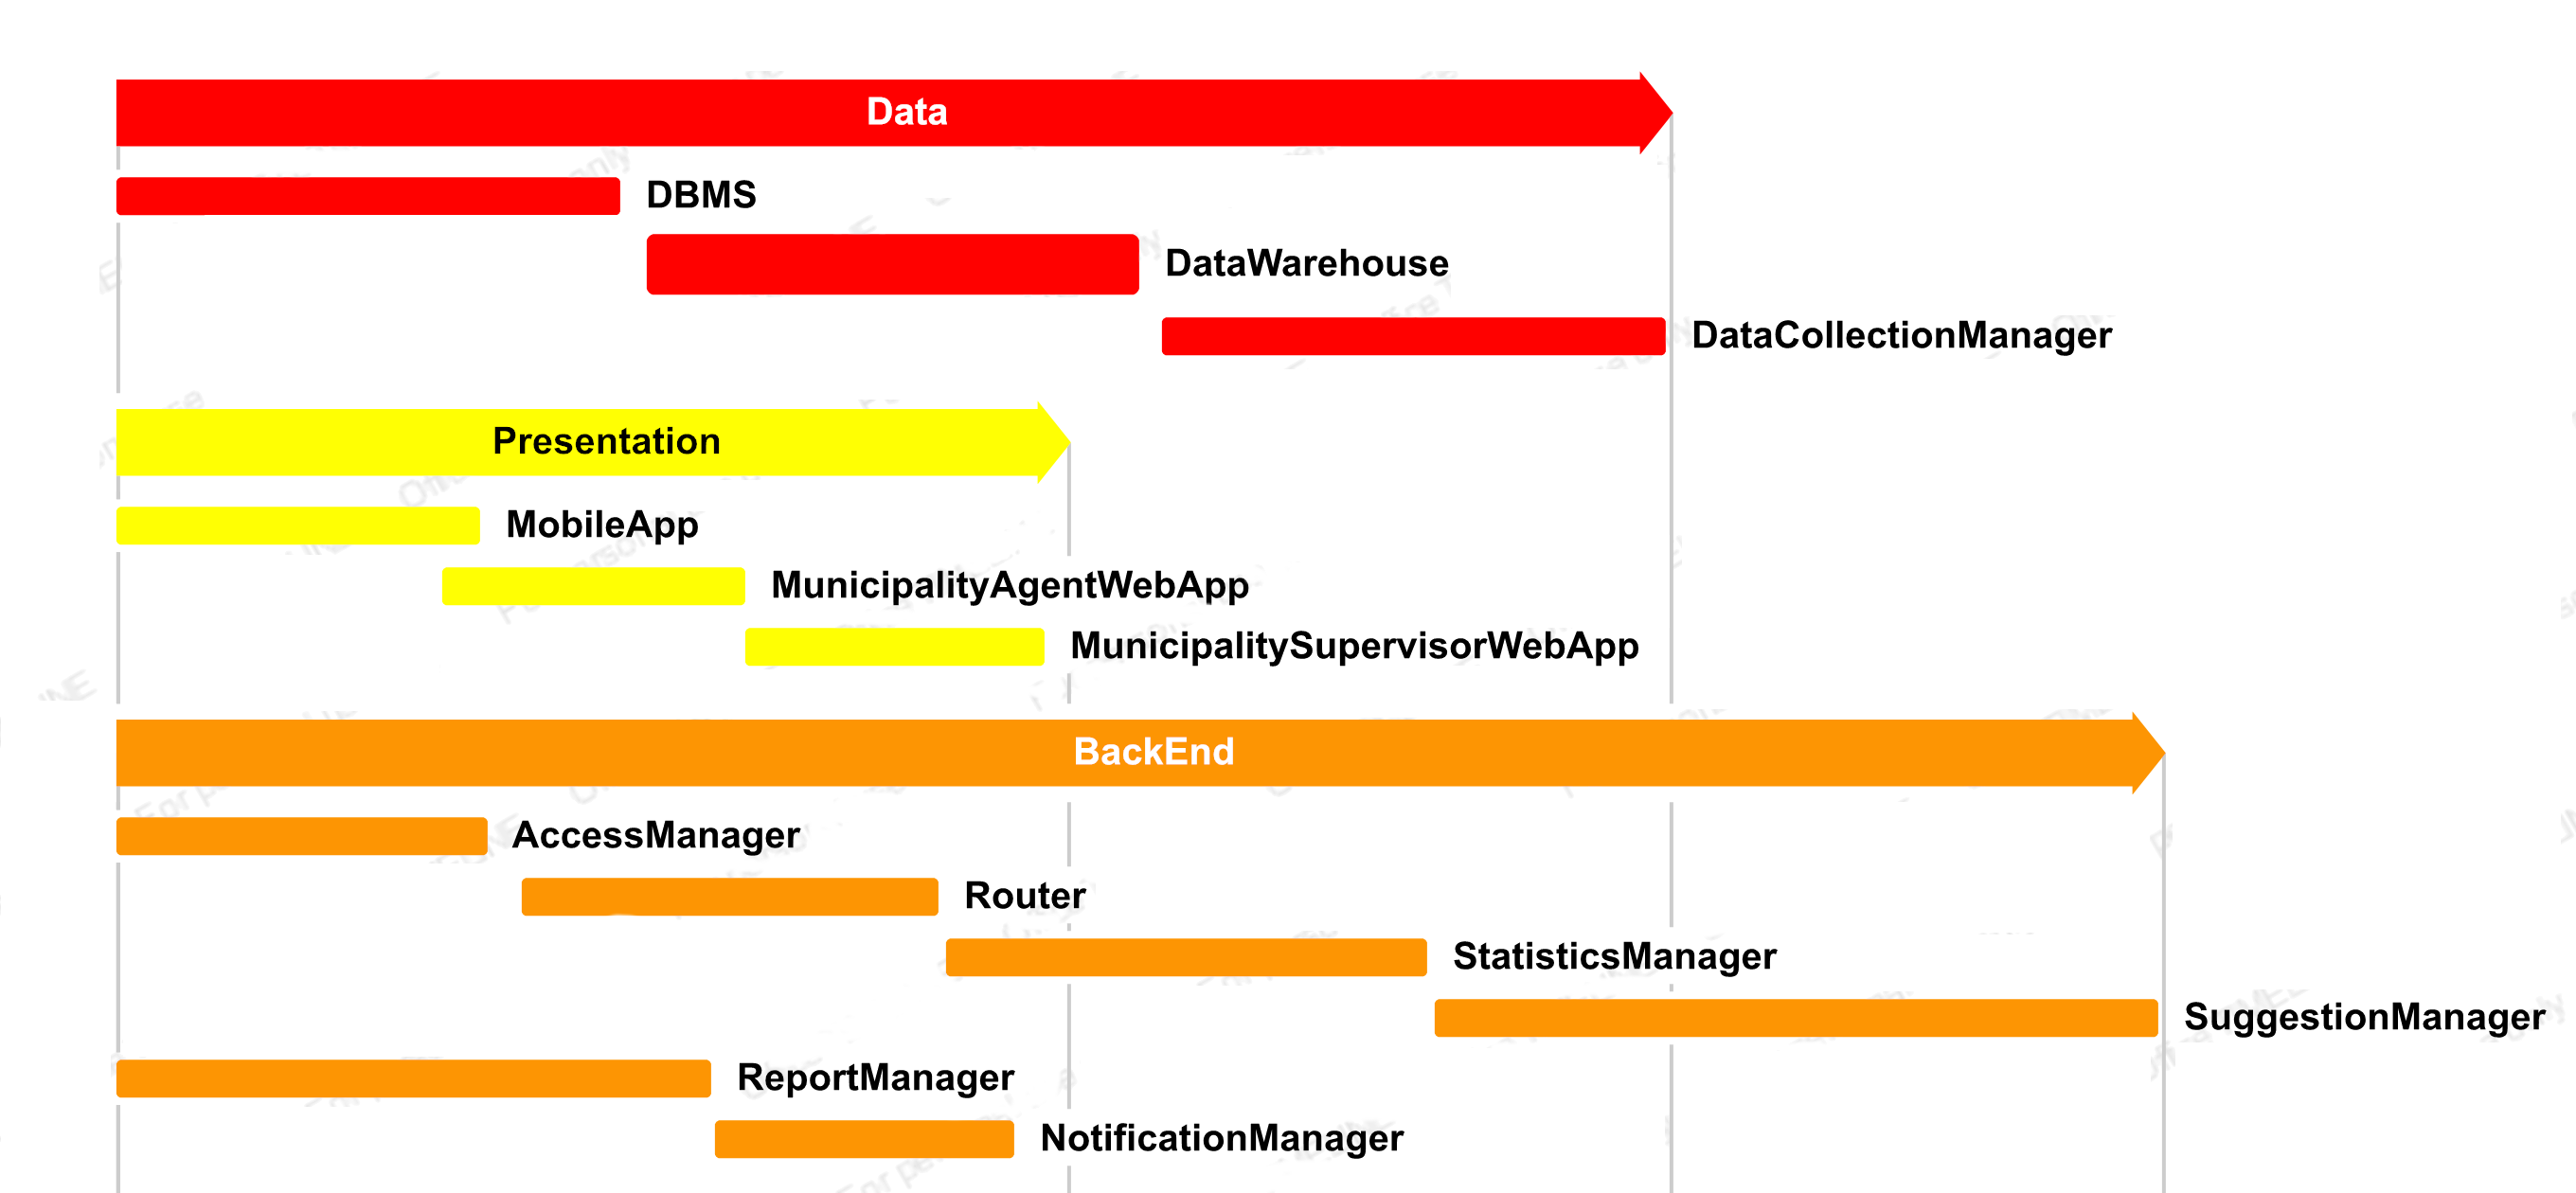
\includegraphics[width=\textwidth]{Gantt2}
\caption{Gantt chart for the implementation process}
\label{fig:gantt}
\end{figure}
All modules need to be tested individually, reaching the 80\% of code coverage. The white testing technique will be adopted for the unit tests and various components will require stubs:
\begin{itemize}
\item \textit{AccessManager}, \textit{ReportManager}, \textit{NotificationManager} will require a stub for the \textit{DBMS}
\item \textit{ReportManager}, \textit{SuggestionManager} will require a stub for the \textit{NotificationManager}
\item \textit{NotificationManager} will require stubs for \textit{UserMobileApp}, \textit{AgentWebApp} and \textit{SupervisorWebApp}
\item \textit{Router} will require stubs for \textit{ReportManager}, \textit{StatisticsManager}, \textit{SuggestionManager}, \textit{AccessManager} and \textit{DBMS}
\end{itemize}
For the \textbf{\textit{AutomaticReportAnalyzer}} subcomponent of the \textit{ReportManager} it will be particularly important to have a large number of tests to ensure to have a discrete level of performance in the identification of fakes.\\
For the \textbf{\textit{MobileApp}} it will be important to test it on various types of mobile devices (smartphones and tablets), with different versions of Android and iOS. The same holds for the \textbf{\textit{WebApps}}, they will need tests on various browsers (\textit{Google Chrome, Mozilla Firefox, Microsoft Edge}), versions and operating systems.
\section{Integration testing}
Once that some modules are completed and tested alone they can be integrated, following a thread-oriented buttom-up order:
\begin{itemize}
\item Once the \textit{DataWarehouse}, the \textit{DataCollectionManager} and the part of \textit{DBMS} related to \textit{streets} are ready they can be integrated (\textit{data collection thread})
\item Once the \textit{ReportManager} the part of \textit{DBMS} related to \textit{reports}, \textit{tickets}, \textit{streets} and \textit{users} and the necessary function of \textit{NotificationManager} are ready they can be integrated  (\textit{report management thread})
\item Once the \textit{AccessManager} and the part of \textit{DBMS} related to \textit{users} are ready, they can be integrated (\textit{access thread})
\item Once the \textit{data collection thread} has been integrated and the \textit{StatisticsManager} is ready, they can be integrated  (\textit{statistics thread})
\item Once the \textit{data collection thread} has been integrated and the \textit{SuggestionsManager} and the necessary function of the \textit{NotificationManager} are ready, they can be integrated (\textit{suggestions thread})
\item Once the \textit{ReportManager}, the \textit{StatisticsManager}, the \textit{AccessManager}, the \textit{SuggestionManager}, the \textit{Router} and the part of \textit{DBMS} related to \textit{users} and \textit{accesses} are ready, they can be integrated (\textit{facade thread})
\item Once the \textit{UserMobileApp}, the \textit{MunicipalityAgentWebApp}, the \textit{SupervisorWebApp} and the \textit{Router} are ready, they can be integrated (\textit{presentation thread})
\item Once the \textit{UserMobileApp}, the \textit{MunicipalityWebApp}, the \textit{SupervisorWebApp} and the \textit{NotificationManager} are ready they can be integrated (\textit{notification thread})
\end{itemize}
The integration test will be black box tests, aim to verify the proper working of all functions in the same way as unit tests, but substituting stubs and drivers with the real corresponding modules.\\
In figures \ref{fig:thread2}, \ref{fig:thread3}, \ref{fig:thread4} and \ref{fig:thread5} the integration threads are highlighted on the component diagram.
\afterpage{
\newgeometry{bottom=2cm}
\begin{landscape}
\begin{figure}[hp]
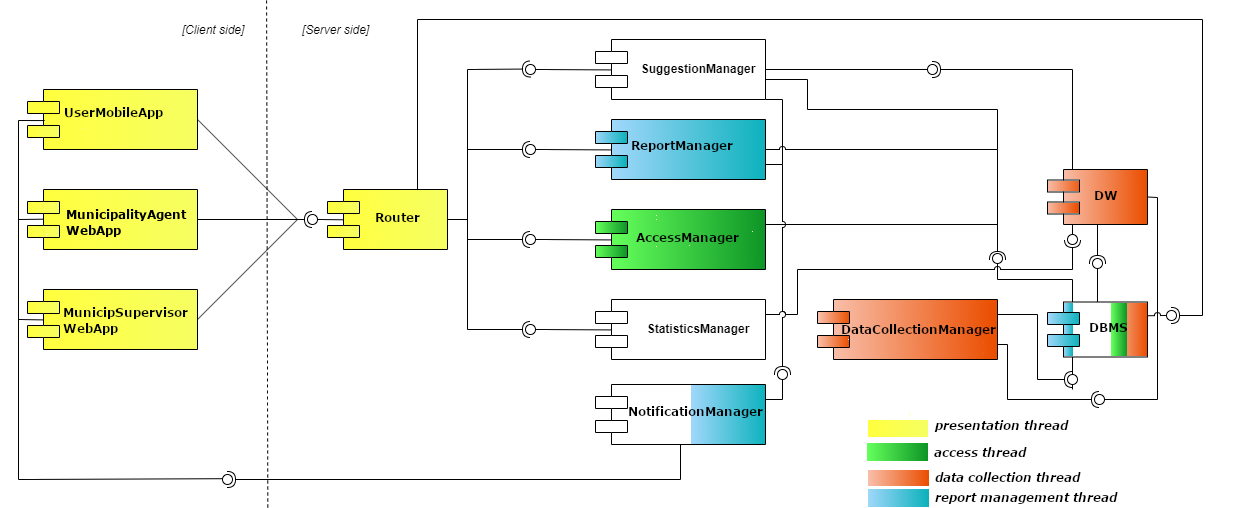
\includegraphics[scale=2.5]{Thread2}
\caption{Integration diagram for access, data collection, report management and presentation}
\label{fig:thread2}
\end{figure}
\end{landscape}
\restoregeometry
}
\begin{figure}[htp]
\centering
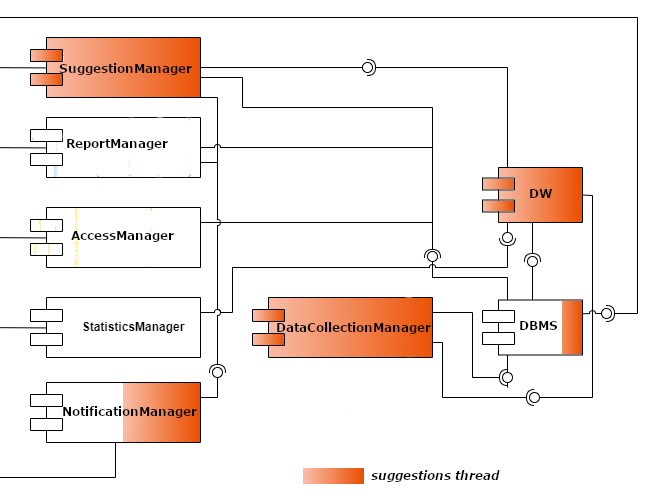
\includegraphics[scale=2]{Thread3}
\caption{Integration diagram for suggestions}
\label{fig:thread3}
\end{figure}

\begin{figure}[htp]
\centering
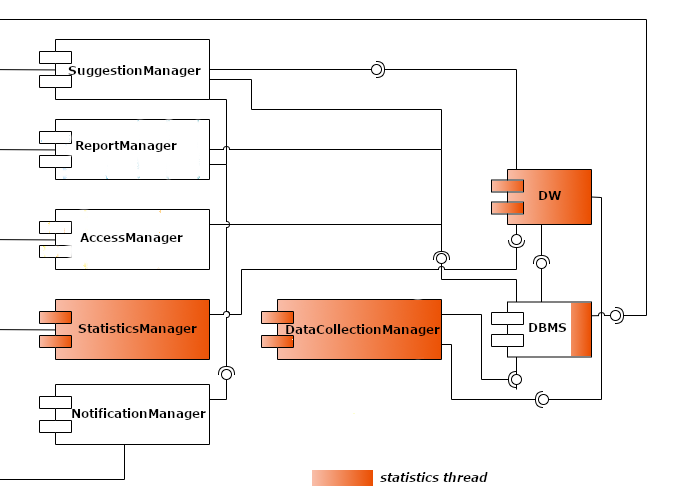
\includegraphics[scale=2]{Thread4}
\caption{Integration diagram for statistics}
\label{fig:thread4}
\end{figure}

\afterpage{
\newgeometry{bottom=2cm}
\begin{landscape}
\begin{figure}[hp]
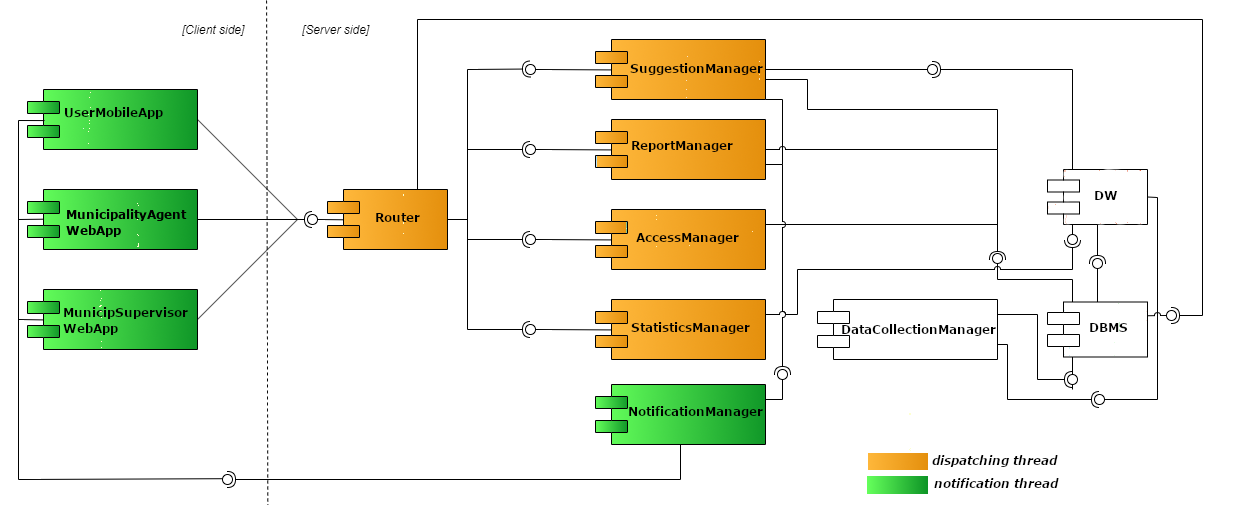
\includegraphics[scale=2.5]{Thread5}
\caption{Integration diagram for dispatching and notification}
\label{fig:thread5}
\end{figure}
\end{landscape}
\restoregeometry
}

\section{System testing}
After the integration testing the system must be subjected to system tests.\\
First of all the system will be subjected to an \textit{\textbf{alpha test}}, executed by the \textit{SafeStreets} developers in their production environment, checking all functions with a good numbers of test cases (it should be checked that they cover at least 80\% of the code).\\
After the check of the \textbf{functional} requirements this test will also verify the \textbf{non-functional} requirements, in particular the performances under an heavy load: the database and the datawarehouse will be charged with a big quantity of data (similar to the expected data for tens of municipality in a decade) and all functions will be tested, checking their elaboration and response times.\\
The second and most important system test is the \textit{\textbf{beta test}}, which will be executed in a real production environment, with the support of a municipality: a group of voluntary citizens will install and try the mobile app, while a selected group of agents and supervisors will use web apps.\\
This is particular important to verify another time the correct behavior of the system (i.e. the absence of bugs), in a real distributed environment, but also to verify the \textbf{usability} of the system and the correctness w.r.t to the needs of the various types of users (\textbf{acceptance test}).


\chapter{Effort spent}

\begin{table}[H]
\centering
Nicola Rosetti \\
%\begin{tabular}{lll}
\begin{tabular}{p{2cm}p{1.5cm}p{7cm}}
\toprule
\textit{Date} & \textit{Hour} & \textit{Section} \\ \midrule
18-11-2019 & 1.5 h* & Component and high-level architecture analysis \\ \midrule
21-11.2019 & 1.5 h & Other design decision part: consistency and replication \\ \midrule
23-11-2019 & 2 h & Introduction and high-level architecture in chap 2 \\ \midrule
25-11-2019 & 3 h & Requirements traceability \\ \midrule
27-11-2019 & 1 h & Runtime View \\ \midrule
28-11-2019 & 1 h* & RASD Update \\ \midrule
29-11-2019 & 3 h & Requirements traceability \\ \midrule
29-11-2019 & 2 h & Chapter 1 introduction \\ \midrule
29-11-2019 & 1 h & Deployment view \\ \midrule
1-12-2019 & 2 h & Mockup and general revision \\ \midrule
2-12-2019 & 2 h & Selected architectural styles and patterns section \\ \midrule
3-12-2019 & 1.5 h & Chapter 3 and activity diagram \\ \midrule
4-12-2019 & 1 h & activity diagrams \\ \midrule
5-12-2019 & 1 h* & minor updates and fixes\\ \midrule
7-12-2019 & 1 h & activity diagrams \\ \midrule
7-12-2019 & 1 h & RASD update\\ \midrule
8-12-2019 & 1 h & general revision\\ \midrule
\bottomrule
\end{tabular}
\caption[Nicola Rosetti's effort table]{}
\end{table}


\vspace*{1 cm}
\begin{table}[H]
\centering
Simone Sartoni \\
\begin{tabular}{p{2cm}p{1.5cm}p{7cm}}
\toprule
\textit{Date} & \textit{Hour} & \textit{Section} \\ \midrule
18-11-2019 & 1.5  h* & Componenst and high-level architecture analysis \\ \midrule
24-11-2019 & 2.5 h &  System architecture diagram \\ \midrule
24-11-2019 & 1.5 h &  Deployment diagram\\ \midrule
27-11-2019 & 1.5 h & Update deployment diagram, requirements traceability revision and Requirements Traceability Matrix creation \\ \midrule
28-11-2019 & 3 h & Requirements Traceability Matrix update and Interface Diagram \\ \midrule
29-11-2019 & 1.5 h & Components Interface Diagram \\ \midrule
03-11-2019 & 3 h & Components Interface Diagram update \\ \midrule
04-11-2019 & 1.5 h & Components Interface Diagram description \\ \midrule
07-11-2019 & 1.5 h & Minor fixes and changes \\ \midrule
08-11-2019 & 2 h & Chapter 2 final revision and Deployments Diagram update \\ \midrule
09-11-2019 & 1.5 h & Chapter 3 final revision and Component Interfaces Diagram update \\ \midrule
09-11-2019 & 2 h & Chapter 4 final revision\\ \midrule

\bottomrule
\end{tabular}
\caption[Simone Sartoni's effort table]{}
\end{table}
\vspace*{1 cm}
\begin{table}[H]
\centering
Vittorio Torri \\
\begin{tabular}{p{2cm}p{1.5cm}p{7cm}}
\toprule
\textit{Date} & \textit{Hour} & \textit{Section} \\ \midrule
18-11-2019 & 1 h* & Componenst and high-level architecture analysis \\ \midrule
21-11-2019 & 1 h  & Components diagram \\ \midrule
22-11-2019 & 0.5 h & Components diagrams \\ \midrule
23-11-2019 & 1.5 h & Components diagrams and components view\\ \midrule
24-11-2019 & 2 h & Sequence diagrams and components view \\ \midrule
26-11-2019 & 1 h & Sequence diagrams \\ \midrule
27-11-2019 & 1 h & Sequence diagrams \\ \midrule
28-11-2019 & 1 h & Sequence Diagram \\ \midrule
30-11-2019 & 2 h & Mockup \\ \midrule
01-12-2019 & 2 h & Deployment and Runtime View, Scope \\ \midrule
02-12-2019 & 1 h & Implementation and testing \\ \midrule
03-12-2019 & 2 h & Implementation and testing \\ \midrule
04-12-2019 & 1 h & Integration diagrams \\ \midrule
05-12-2019 & 1 h* & Minor changes and fixes \\ \midrule
06-12-2019 & 1.5 h & E/R and DFM diagrams \\ \midrule
07-12-2019 & 2 h & Web Registration mockup, gantt chart \\ \midrule
07-12-2019 & 1 h & Class diagram update and minor fixes \\ \midrule
08-12-2019 & 1 h & Minor fixes \\
\bottomrule
\end{tabular}
\caption[Vittorio Torri's effort table]{}
\end{table}
\textit{* Group work}

\chapter{References}

\begin{itemize}
\item \label{ref:facade-pattern} \hyperref[use:facade-pattern]{\textit{[FACADE-PATTERN]}}\href{https://en.wikipedia.org/wiki/Facade\_pattern}{\textit{https://en.wikipedia.org/wiki/Facade\_pattern}} - definition of facade pattern
\item \label{ref:MVC-pattern} \hyperref[use:MVC-pattern]{\textit{[MVC-PATTERN]}}\href{https://en.wikipedia.org/wiki/Model\%E2\%80\%93view\%E2\%80\%93controller}{\textit{https://en.wikipedia.org/wiki/Model\%E2\%80\%93view\%E2\%80\%93controller}} - definition of MVC pattern
\item \label{ref:RESTful-architecture} \hyperref[use:RESTful-architecture]{\textit{[RESTFUL-ARCHITECTURE]}}\href{https://restfulapi.net/rest-architectural-constraints/}{\textit{https://restfulapi.net/rest-architectural-constraints/}}- definition and characteristics of RESTful architecture
\item \label{ref:UML-Activity} \hyperref[use:UML-Activity]{\textit{[UML-ACTIVITY]}}\href{https://www.academia.edu/5041934/User\_Interface\_Modelling\_with\_UML}{\textit{https://www.academia.edu/5041934/User\_Interface\_Modelling\_with\_UML}}- User Interfaces Modelling using UML, Pinheiro Paulo, Paton Norman, 2002/11/23
\item \label{ref:pubsub-pattern} \hyperref[use:pubsub-pattern]{\textit{[PUBSUB-PATTERN]}}\href{https://en.wikipedia.org/wiki/Publish\%E2\%80\%93subscribe\_pattern}{\textit{https://en.wikipedia.org/wiki/Publish\%E2\%80\%93subscribe\_pattern}}- Wikipedia page for publish - subscribe pattern
\end{itemize}
\end{document}
